\chapter{Introducción específica} % Main chapter title

\label{Chapter2}

%----------------------------------------------------------------------------------------
%	SECTION {Funcionamiento general del sistema}
%----------------------------------------------------------------------------------------
\section{Funcionamiento general del sistema}

En este capítulo se exponen las características del software utilizado para la programación del sistema, partiendo del backend hasta el frontend. También se identifican los módulos de funcionamiento del dispositivo conversor Modbus a MQTT para utilizar en el trabajo.  Finalmente se describe la utilidad de Nginx como servidor de datos para integrar el sistema. 



%----------------------------------------------------------------------------------------
%	SECTION {Dispositivo conversor Modbus a MQTT}
%----------------------------------------------------------------------------------------
\section{Dispositivo conversor Modbus a MQTT}

El conversor consta de un circuito electrónico que actúa de interfaz de conexión entre aparatos o dispositivos que se encuentran en una red Modbus y posibilita la conversión de datos al protocolo MQTT a través de una conexión .

En la figura \ref{fig:dev-conv} se puede observar el diagrama de bloques con las partes mas importantes que componen al dispositivo. 

\begin{figure}[htpb]
	\centering
	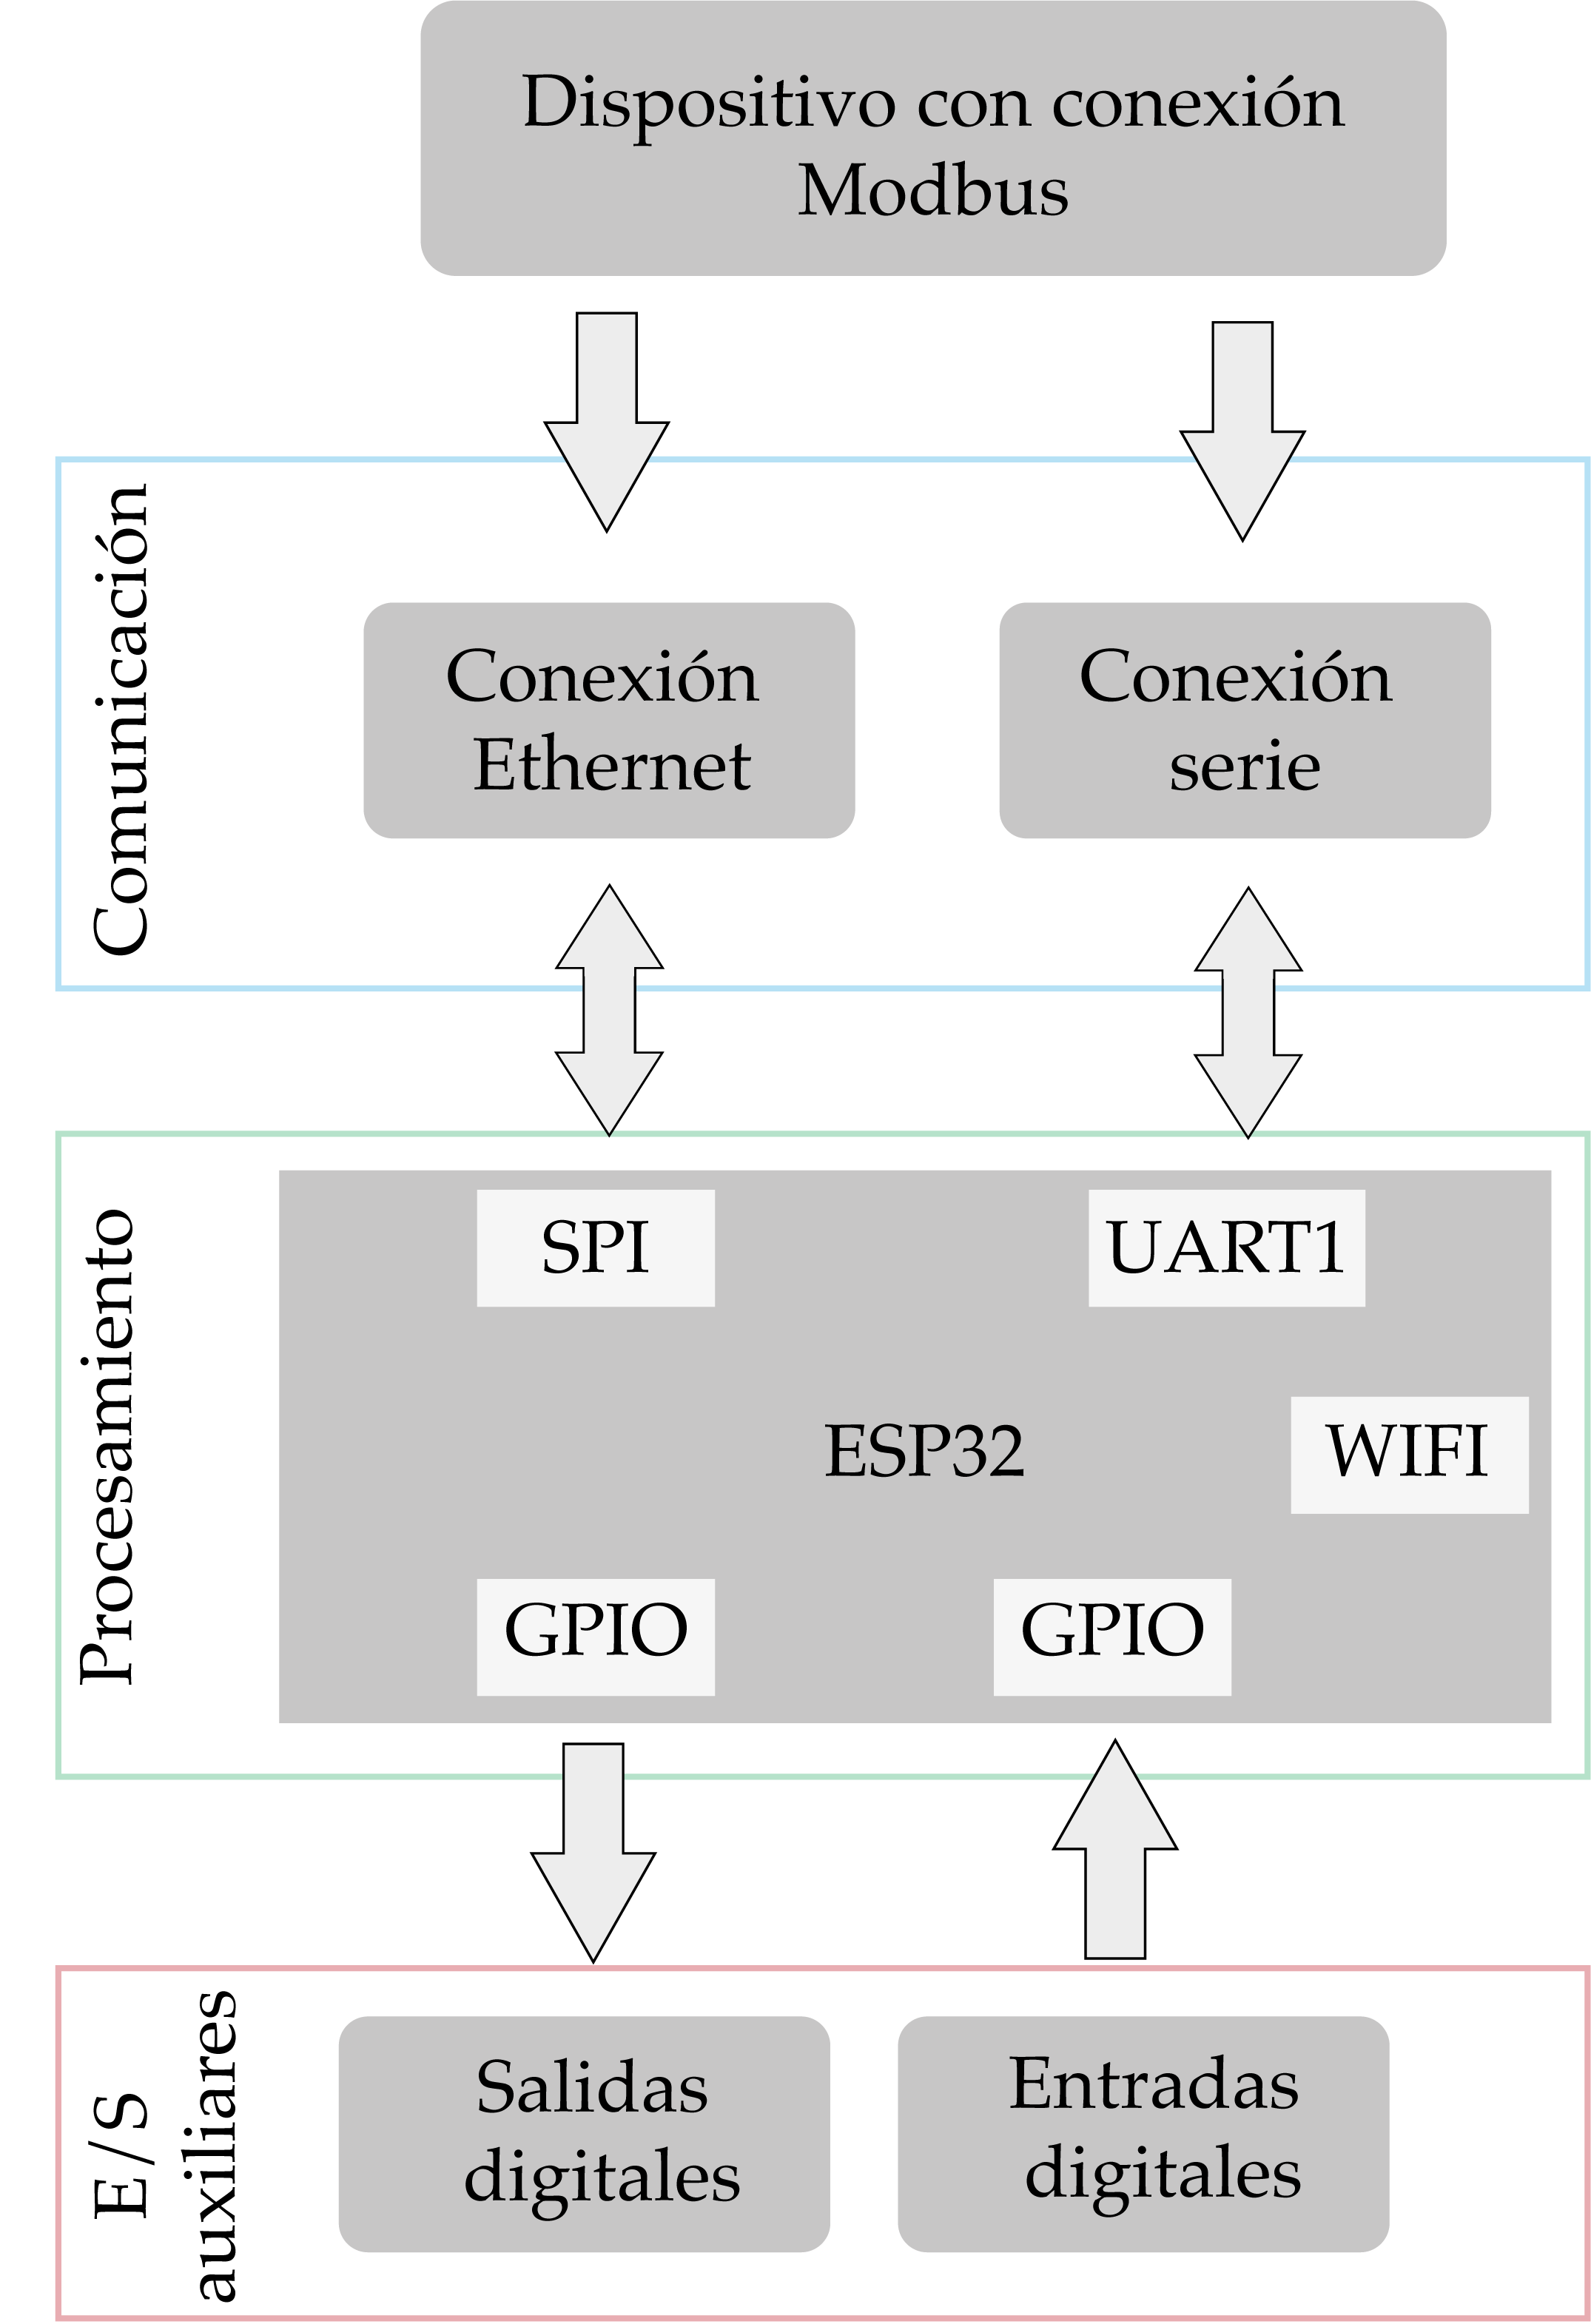
\includegraphics[scale=.35]{./Figures/diagrama_dispositivo.png}
	\caption[Diagrama de bloques de dispositivo conversor ]{Diagrama de bloques de dispositivo conversor Modbus a MQTT.}
	\label{fig:dev-conv}
\end{figure}

Al sistema se lo puede separar en tres grupos:

\begin{itemize}
	\item Comunicación: este bloque está compuesto por un circuito de conexión ethernet para poder recibir mensajes de dispositivos que están conectados a través de Modbus TCP. 
	
	Por otro lado el hardware contiene un circuito de conexión para dispositivos que se conectan por Modbus serie.
	
	\item Procesamiento: es el bloque principal donde se gestionan todos los datos recibidos por parte del módulo de comunicación y  convierte los mensajes Modbus para luego poder ser enviados por MQTT a través de wifi.  
	
	Este módulo está constituido por un microcontrolador ESP32 \citep{WEBSITE:11} de la empresa Espressif \citep{WEBSITE:10} quien se encarga de controlar el módulo de comunicación y el módulo de entradas y salidas auxiliares.
	
	Los datos provenientes del módulo de comunicación son reconvertidos a un formato de datos del tipo JSON \citep{WEBSITE:12} para ser enviados vía wifi por protocolo MQTT.
	
	
	\item Entradas y salidas auxiliares: este bloque permite conectar dispositivos externos al conversor. 
	
	Como ejemplo se pueden mencionar sensores para las entradas y actuadores para las salidas. 
	
	
\end{itemize}


%----------------------------------------------------------------------------------------
%	SECTION {Protocolos}
%----------------------------------------------------------------------------------------
\section{Protocolos de comunicación}
En el caso de la comunicación con un servidor remoto, se requiere tener acceso a Internet y por lo tanto es necesario conectarse también con un módem, que a
su vez debe estar conectado a un proveedor de servicios de Internet (ISP, por sus siglas en inglés correspondientes a \textit{Internet Service Provider} ).

Necesariamente para poder conectarse a Internet, el conversor de protocolo Modbus a MQTT debe implementar el protocolo TCP/IP\citep{WEBSITE:15} o UDP/IP,\citep{WEBSITE:16} que determinan las características de las capas de transporte y red del estándar OSI \citep{WEBSITE:13} respectivamente. La capa de aplicación, ubicada en la parte superior del modelo, es la encargada de ofrecer a las aplicaciones de usuario la posibilidad de comunicarse con otros dispositivos a través de los servicios brindados por las demás capas. Entre los protocolos de aplicación, existen múltiples como AMQP, CoAP, DDS, STOMP, MQTT y HTTP, siendo estos dos últimos los utilizados en el trabajo realizado.

Ambos protocolos son ampliamente utilizados para aplicaciones en la internet de las cosas.  MQTT se basa en un modelo de publicaciones y suscripciones, en el que un cliente publica mensajes en un tema o tópico, y todos aquellos nodos que se encuentran suscritos a ese tema reciben el mensaje publicado. MQTT es ideal para aplicaciones de IoT, debido principalmente a que requiere un muy bajo ancho de banda, tiene un menor consumo de potencia que otras alternativas, y además es sencillo y ligero de implementar. 

Por otro lado, HTTP \citep{WEBSITE:14} (\textit{ Hypertext Transfer Protocol} ) nos permite realizar una petición de datos y recursos, como pueden ser documentos HTML \citep{BOOK:2} y es la base de cualquier intercambio de datos en la web. La estructura está basada en cliente y servidor, esto quiere decir que una petición de datos es iniciada por el elemento que recibirá los datos (el cliente), normalmente un navegador web.   Así,  una página web completa resulta de la unión de distintos sub documentos recibidos, como ser un documento que especifique el estilo de maquetación de la página web, el texto, las imágenes, vídeos, scripts, entre otros. 

Clientes y servidores se comunican intercambiando mensajes individuales. Los mensajes que envía el cliente, se llaman peticiones, y los mensajes enviados por el servidor se llaman respuestas.


%----------------------------------------------------------------------------------------
%	SECTION {MQTT}
%----------------------------------------------------------------------------------------
\subsection{Protocolo MQTT}
\label{mqtt-section}
MQTT o \textit{ Message Queue Telemetry Transport}, es un protocolo de transporte liviano de mensajes basado en un modelo de publicaciones y suscripciones, como se ilustra en la figura \ref{fig:mqtt-esquema}. El protocolo MQTT funciona sobre TCP/IP o sobre otros protocolos de red con soporte bidireccional y sin pérdidas de datos.

\begin{figure}[htpb]
	\centering
	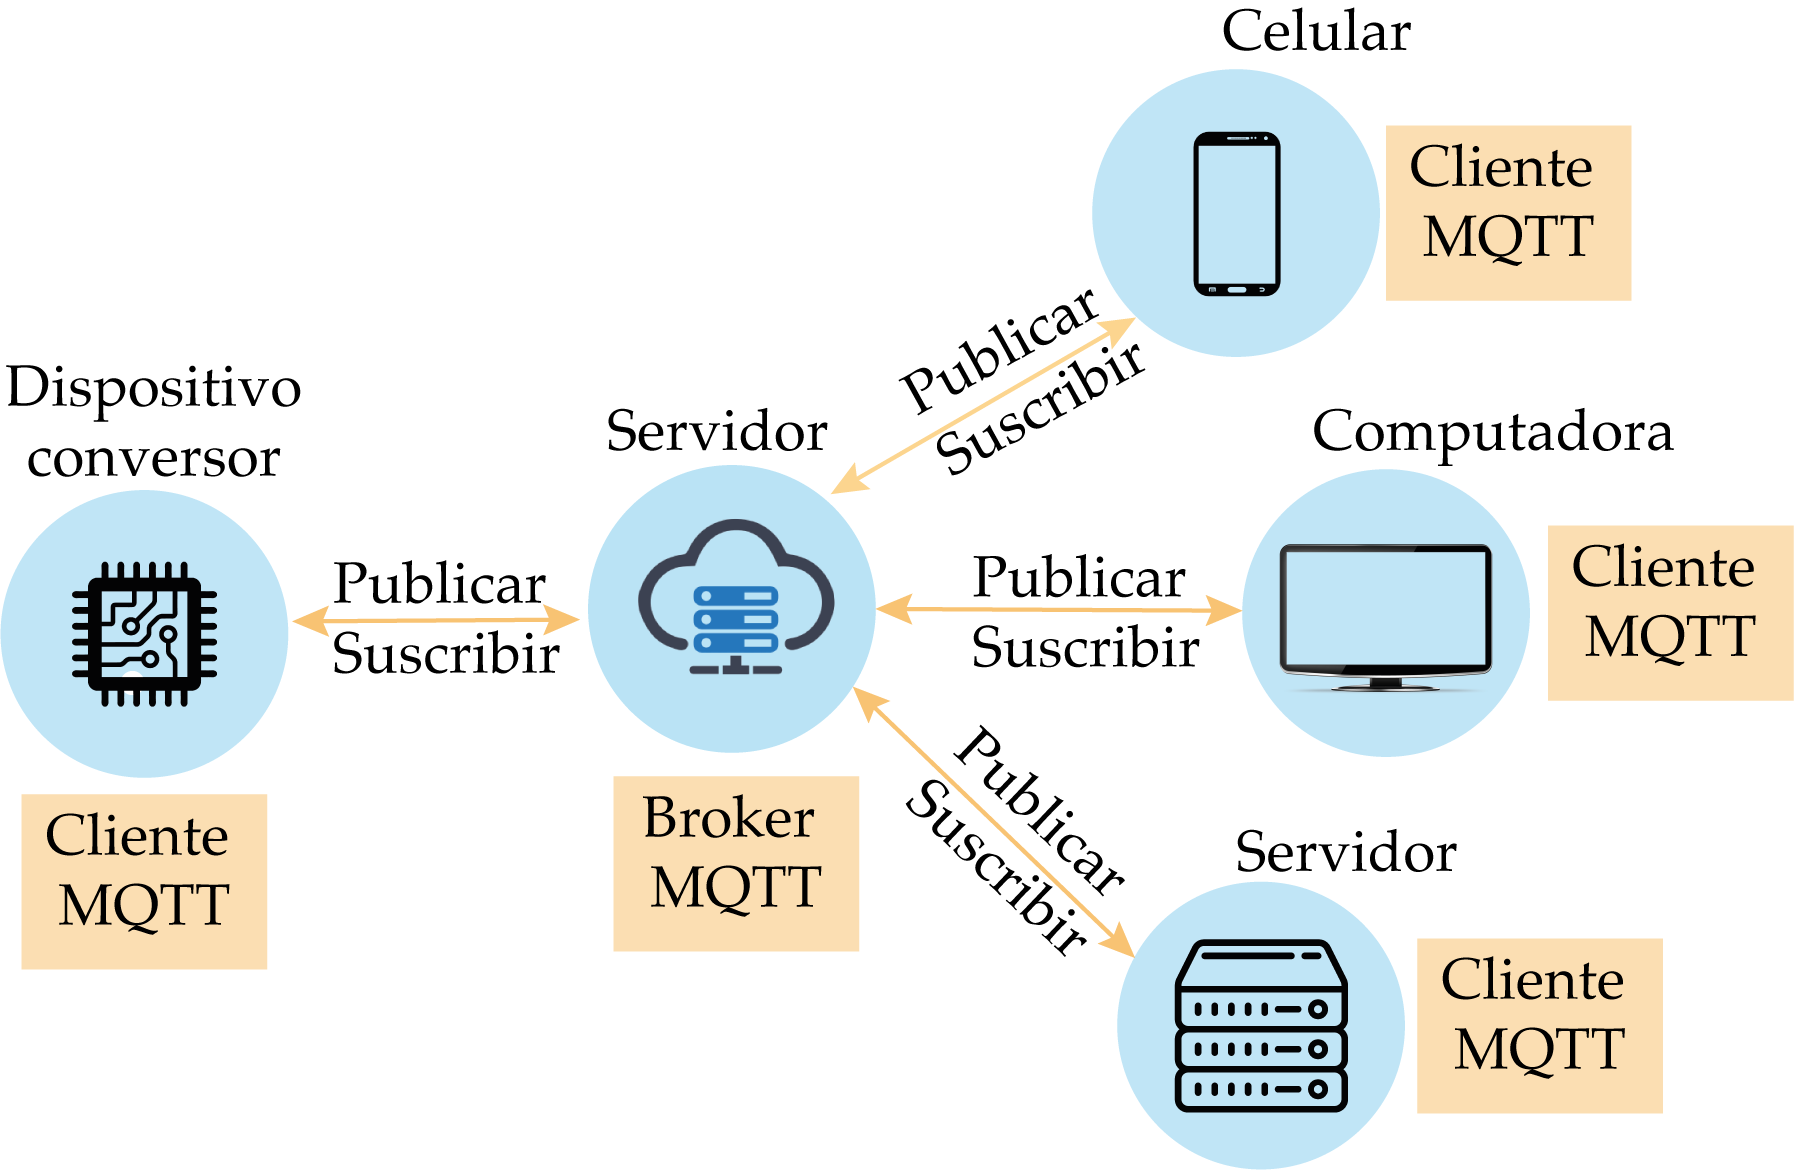
\includegraphics[scale=.7]{./Figures/mqtt-protocol.png}
	\caption[Esquema de funcionamiento MQTT ]{Modelo de funcionamiento de protocolo MQTT.}
	\label{fig:mqtt-esquema}
\end{figure}

En modelos del tipo publicación y suscripción, un dispositivo puede publicar un mensaje en un tema o tópico y/o suscribirse a un tópico particular para la recepción de mensajes.  A diferencia de un modelo cliente/servidor típico donde ambas partes se comunican directamente, en este esquema se desacopla tanto el cliente que envía un mensaje, como él o los clientes que están suscritos a dicho tópico y reciben ese mensaje. 

La conexión entre ambas partes es manejada por una tercera parte llamada broker MQTT.  El broker MQTT es el responsable de recibir todos los mensajes, filtrarlos y distribuirlos según corresponda, es decir determinar qué cliente está suscrito a cada tópico y enviar los mensajes publicados en ellos a estos suscriptores.

La conexión en MQTT es siempre entre un cliente y el broker, como se ilustra en la figura \ref{fig:mqtt-cliente-broker} es decir que los clientes nunca se conectan entre ellos directamente.

\begin{figure}[htpb]
	\centering
	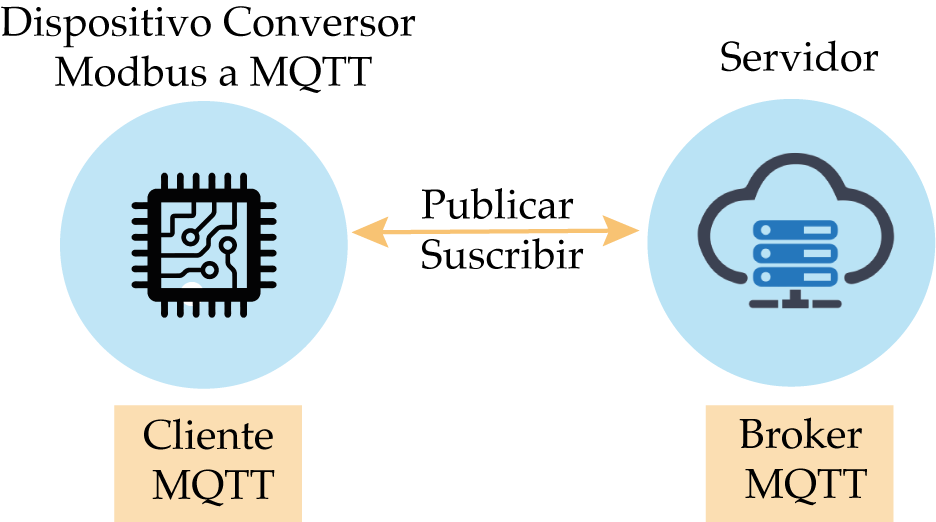
\includegraphics[scale=.7]{./Figures/cliente-broker.png}
	\caption{Esquema de conexión cliente - broker MQTT.}
	\label{fig:mqtt-cliente-broker}
\end{figure}

Para iniciar una conexión, el cliente envía un mensaje CONNECT al broker y este responde con un mensaje CONNACK y un código de estado. Una vez que la conexión queda establecida, el broker la mantiene abierta hasta que el cliente envía un comando de desconexión o la conexión se pierde por algún motivo. Los puertos estándar son 1883 para comunicación no encriptada y 8883 para comunicación encriptada usando SSL/TLS \citep{WEBSITE:17}.

Durante el handshake SSL/TLS, el cliente valida el certificado del servidor para autenticarlo. El cliente puede también proveer un certificado al broker durante el handshake, que el broker utilizará para autenticar al cliente. Si bien no es parte de la especificación, se ha vuelto habitual que los brokers admitan la autenticación de clientes con certificados SSL/TLS. Debido a que el protocolo MQTT apunta a ser un protocolo para dispositivos de IoT con recursos limitados, SSL/TLS puede no ser siempre una opción y, en algunos casos, puede que no sea deseable. En tales casos, la autenticación se presenta como un nombre de usuario y una contraseña de texto simple que el cliente envía al servidor como parte de la secuencia de paquetes CONNECT/CONNACK.  En el caso del presente trabajo, se optó utilizar autenticación mediante nombre de usuario y contraseña y certificado SSL para el cliente web.

Los mensajes son la información que se quiere intercambiar entre los dispositivos, ya sean comandos o datos. En MQTT la palabra tópico refiere a una cadena de caracteres que el broker utiliza para filtrar mensajes para cada cliente conectado. Los tópicos consisten en uno o más niveles. Cada nivel de tópico está separado por una barra. Existen algunos caracteres reservados que son utilizados como comodines o \textit{wildcards} que permiten la suscripción a múltiples tópicos, como el carácter '+' y el carácter '\#', que representan el  \textit{wildcards} de nivel único y de nivel múltiple, respectivamente. En cualquier caso, no es necesario que los clientes creen previamente el tópico antes de publicar o suscribirse a él. El broker acepta cada tópico válido sin previa inicialización.

Ejemplos de tópicos y uso de los wildcards son provistos en la figura \ref{fig:mqtt-wildcards}:

\begin{figure}[htpb]
	\centering
	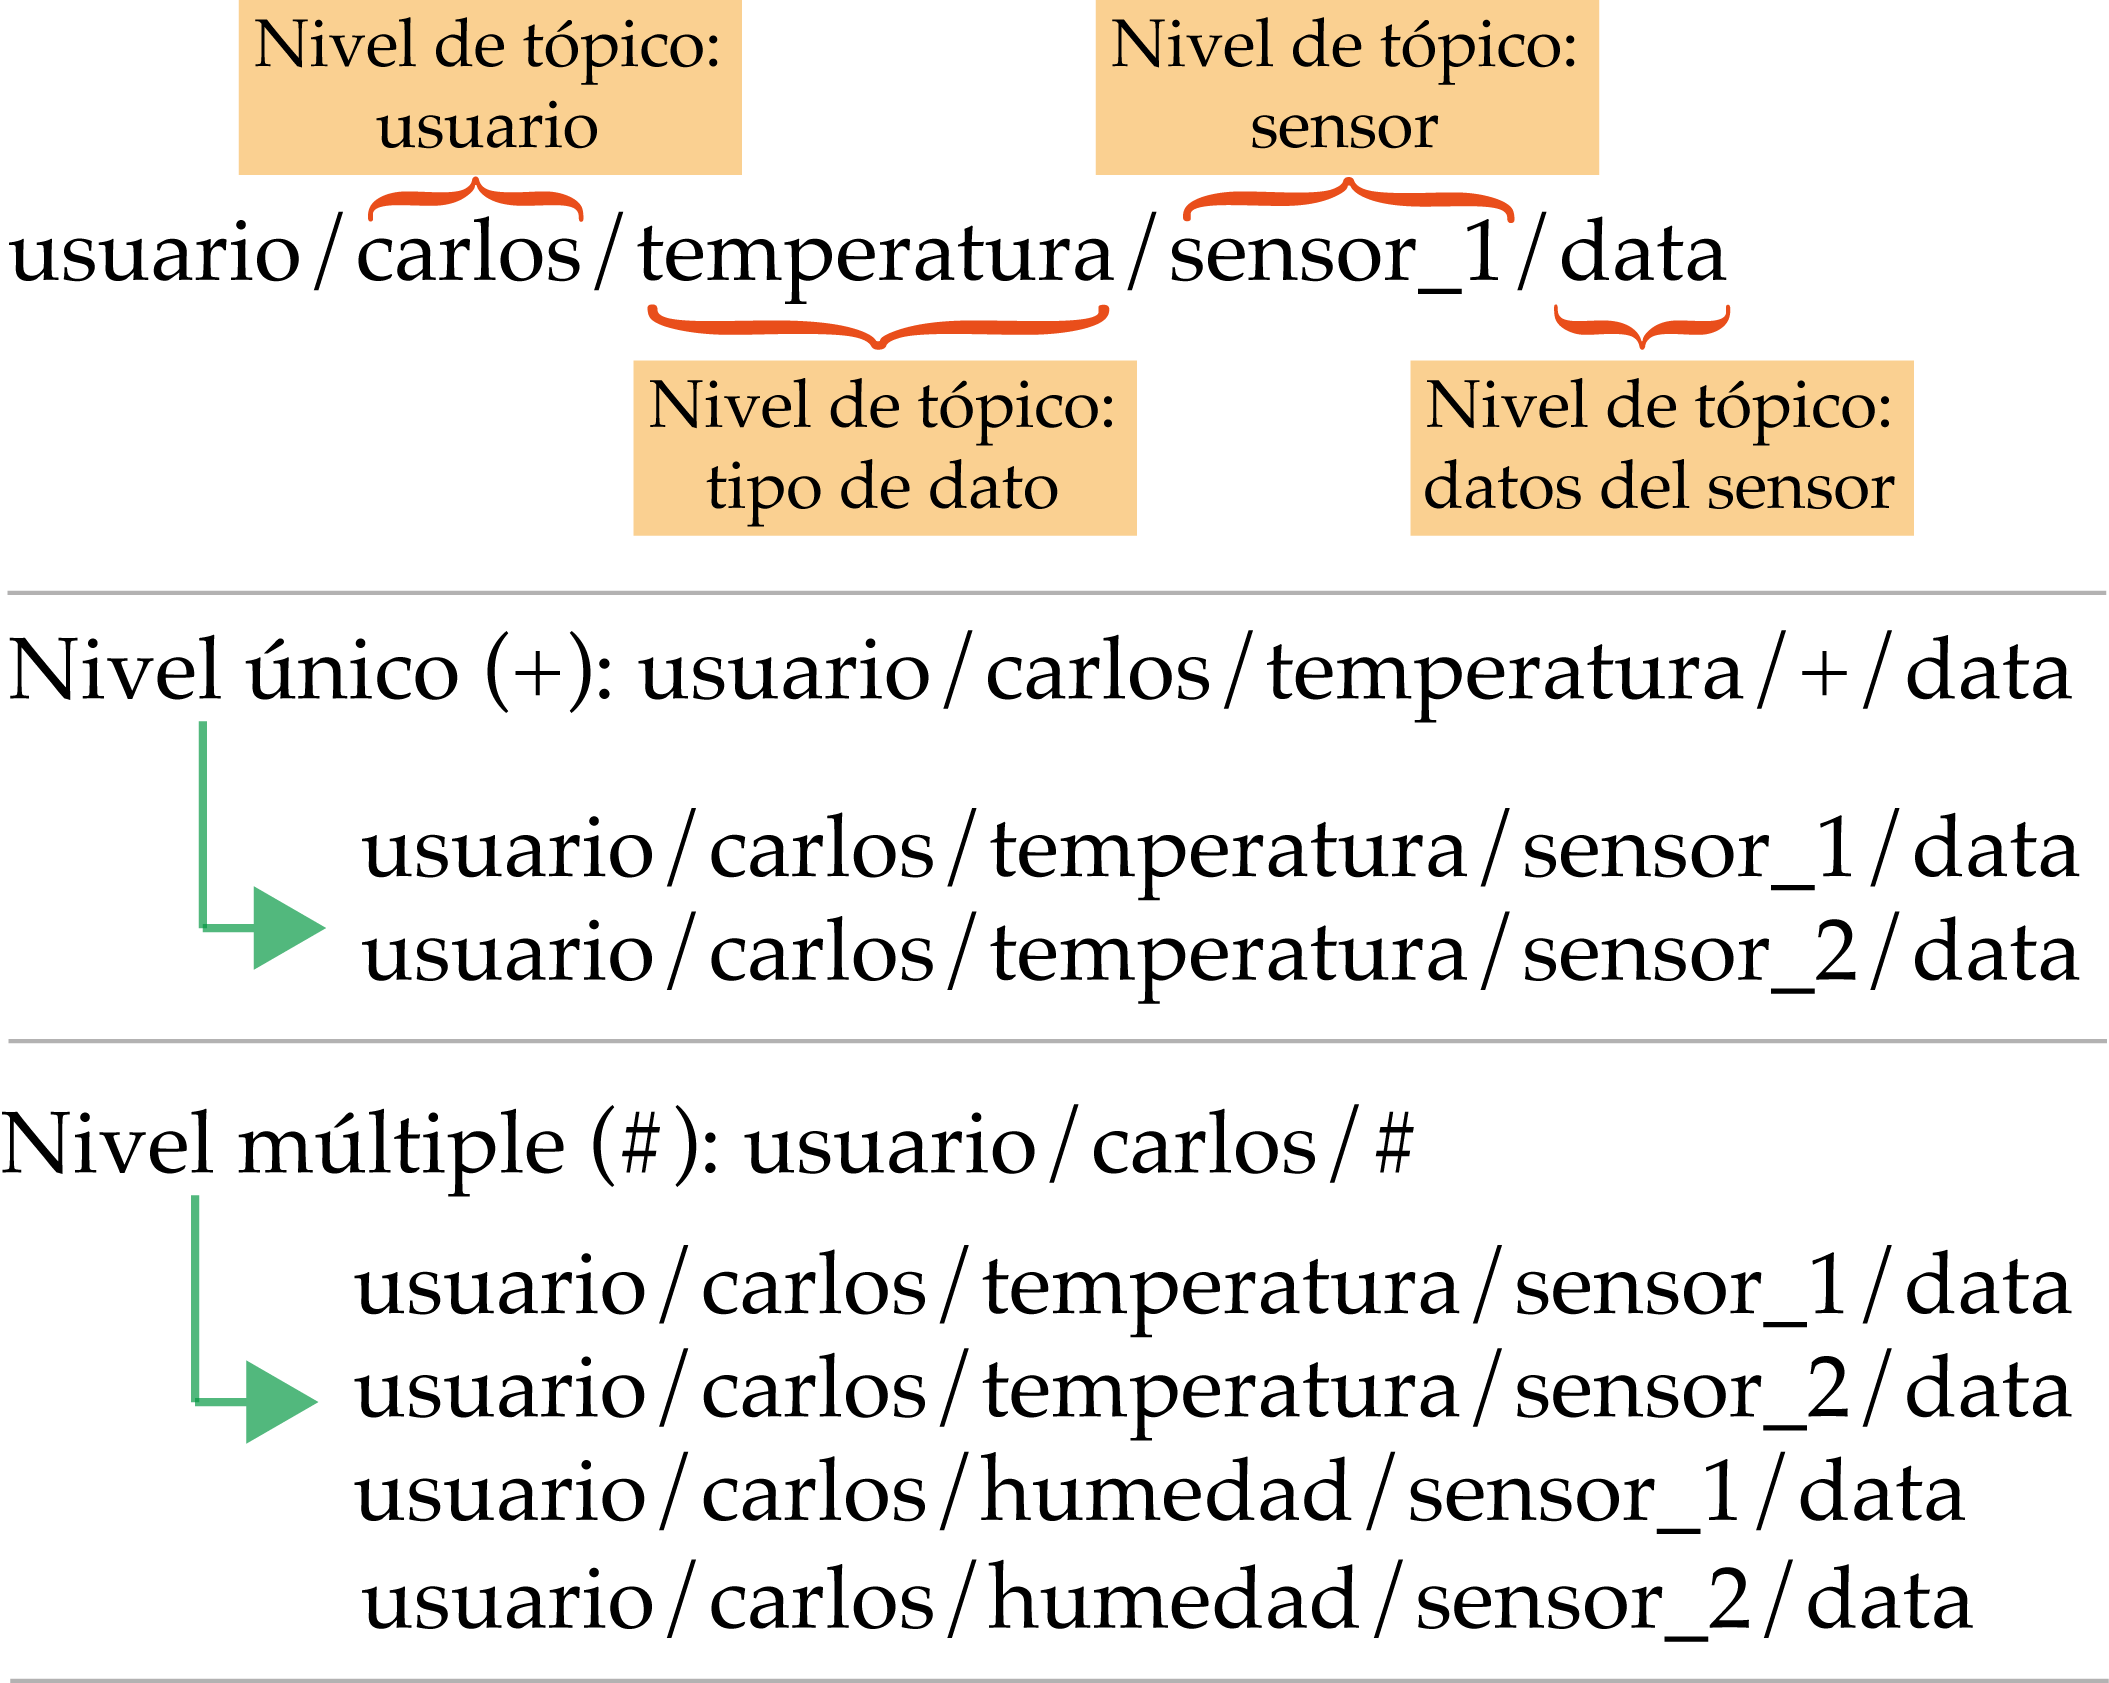
\includegraphics[scale=.38]{./Figures/esquema-wildcard.png}
	\caption{Ejemplo de tópicos y uso de \textit{wildcards}.}
	\label{fig:mqtt-wildcards}
\end{figure}



%----------------------------------------------------------------------------------------
%	SECTION {Protocolo HTTP}
%----------------------------------------------------------------------------------------
\subsection{Protocolo HTTP}

Diseñado a principios de la década de 1990, HTTP es un protocolo ampliable, que ha ido evolucionando con el tiempo. Es lo que se conoce como un protocolo de la capa de aplicación, y se transmite sobre el protocolo TCP, o el protocolo encriptado TLS, aunque teóricamente podría usarse cualquier otro protocolo fiable. 

Gracias a que es un protocolo capaz de ampliarse, se usa no solo para transmitir documentos de hipertexto (HTML), si no que además se usa para transmitir imágenes o vídeos, o enviar datos o contenido a los servidores, como en el caso de los formularios de datos. HTTP puede incluso ser utilizado para transmitir partes de documentos, y actualizar páginas web en el acto.

Es un protocolo basado en el principio de cliente-servidor donde las peticiones son enviadas por una entidad llamada agente de usuario (del ingles \textit{user agent}). La mayoría de las veces el agente de usuario o cliente,  es un navegador web. Cada petición individual se envía a un servidor, el cuál la gestiona y responde. Entre cada petición y respuesta, hay varios intermediarios, normalmente denominados proxies \citep{WEBSITE:18} , los cuales realizan distintas funciones, como \textit{gateways} o caches.  En la figura  \ref{fig:server-proxy} se puede visualizar un caso típico de aplicación de utilización de proxy como \textit{gateway}.

\begin{figure}[htpb]
	\centering
	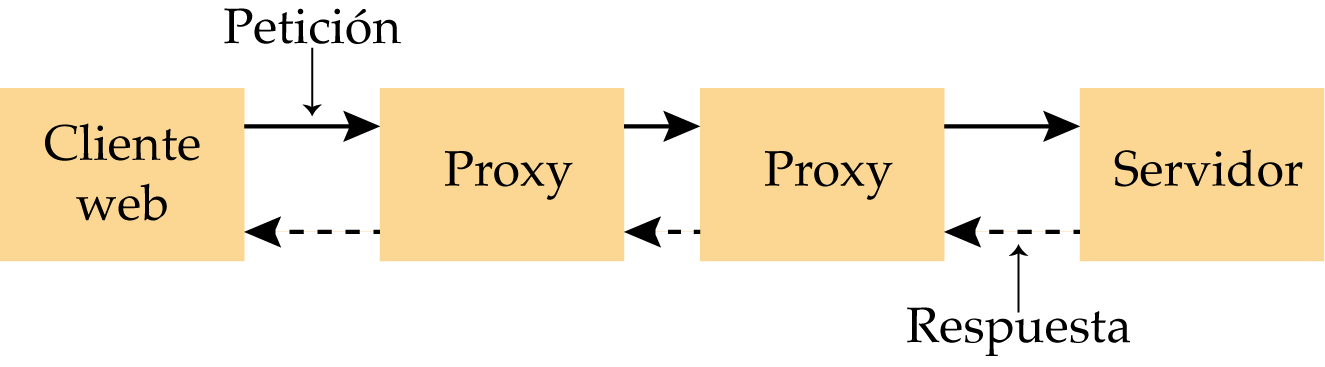
\includegraphics[scale=.80]{./Figures/server-proxy.png}
	\caption[Utilización de proxy como  \textit{gateway}.  ]{Diagrama de bloques ilustrando la utilización de proxy como  \textit{gateway}.}
	\label{fig:server-proxy}
\end{figure}


El navegador es siempre el que inicia una comunicación (petición), y el servidor nunca la comienza, por lo que para poder mostrar una página web, el navegador envía una petición de documento HTML al servidor. Entonces procesa este documento y envía más peticiones para solicitar scripts, hojas de estilo y otros datos que necesite. El navegador, une todos estos documentos y datos y como resultado se obtiene la pagina web. 

Al otro lado del canal de comunicación, está el servidor el cual sirve los datos que ha pedido el cliente. Un servidor conceptualmente es una única entidad, aunque puede estar formado por varios elementos que se reparten la carga de peticiones (\textit{load balancing}), u otros programas que gestionan otras computadoras como cache, bases de datos, servidores de correo electrónico, entre otros y que generan parte o todo el documento que ha sido pedido. 

Una petición de HTTP está formada por los siguientes campos:

\begin{itemize}
	\item Un método HTTP: normalmente pueden ser un verbo, como: GET, POST o un nombre como OPTIONS o HEAD que defina la operación que el cliente quiera realizar. El objetivo de un cliente, suele ser una petición de recursos, usando GET, o presentar un valor de un formulario HTML, usando POST, aunque en otras ocasiones puede hacer otros tipos de peticiones. 
	
	\item La dirección del recurso pedido: la URL del recurso.
	
	\item La versión del protocolo HTTP.
	
	\item Cabeceras HTTP opcionales que pueden aportar información adicional a los servidores.
	
	\item O un cuerpo de mensaje, en algún método como puede ser POST, en el cual envía la información para el servidor.
	
\end{itemize}

A modo de ejemplo, en la figura \ref{fig:peticiones-http}  se puede observar una petición GET al servidor utilizado en este trabajo.

\begin{figure}[htpb]
	\centering
	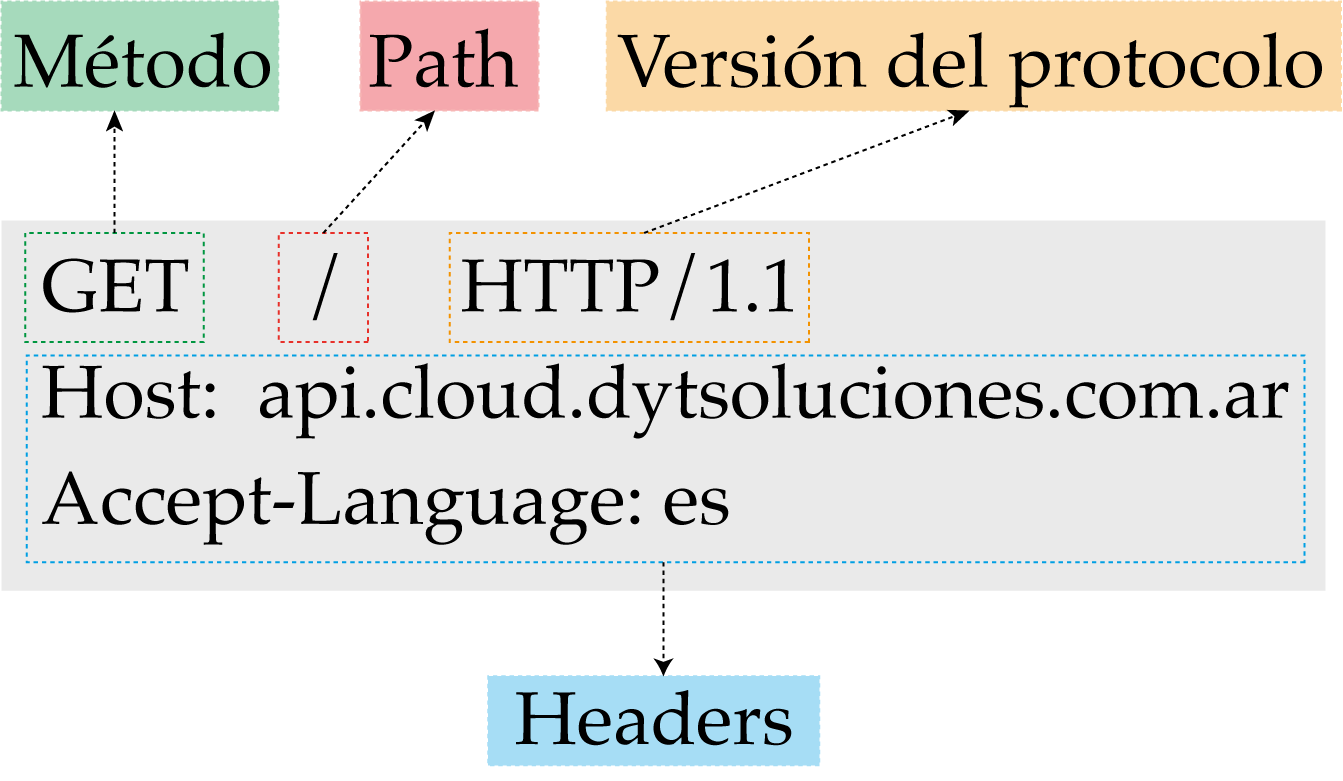
\includegraphics[scale=.50]{./Figures/peticion-http.png}
	\caption[Petición GET al servidor ]{Ejemplo de petición GET al servidor utilizado para realizar este trabajo.}
	\label{fig:peticiones-http}
\end{figure}


Por otro lado, las respuestas están formadas por los siguientes campos:

\begin{itemize}
	\item La versión del protocolo HTTP que se usa.
	
	\item Un código de estado, indicando si la petición ha sido exitosa.
	
	\item Un mensaje de estado, una breve descripción del código de estado.
	
	\item Cabeceras HTTP, como las de las peticiones.
	
	\item Opcionalmente, el recurso que se ha pedido.
	
\end{itemize}

En la figura \ref{fig:respuesta-http}  se observa un modelo de respuesta para ejemplificar los campos mas importantes: 

\begin{figure}[htpb]
	\centering
	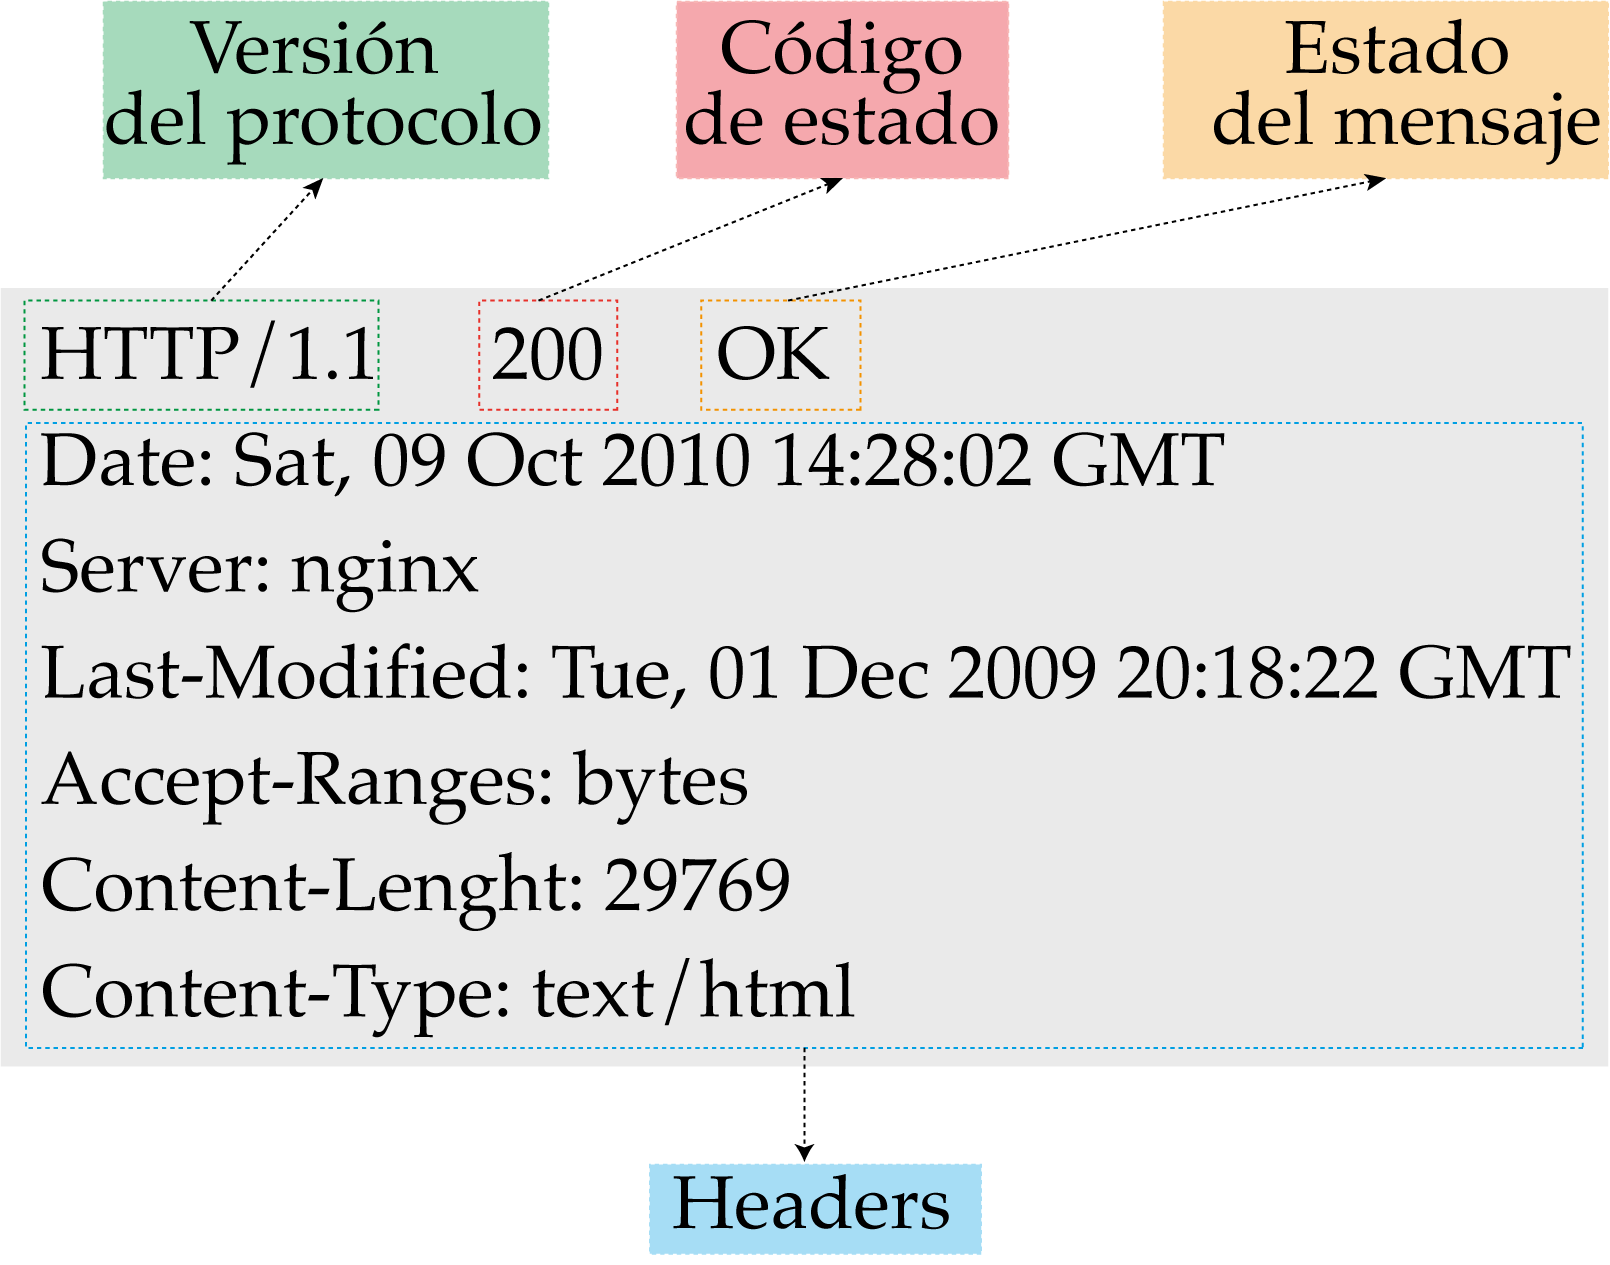
\includegraphics[scale=.50]{./Figures/respuesta-http.png}
	\caption[Modelo de respuesta HTTP ]{Ejemplo de modelo de respuesta HTTP del servidor.}
	\label{fig:respuesta-http}
\end{figure}


%----------------------------------------------------------------------------------------
%	SECTION {Backend}
%----------------------------------------------------------------------------------------
\section{Infraestructura del backend}

En informática, la expresión backend hace referencia a la parte de la infraestructura de datos de un sistema que se encuentran generalmente en el servidor y se encarga de procesar y almacenar información.  Las funciones mas importantes del backend son las siguientes:

\begin{itemize}
	\item Acceder a la información que se pide, a través de la plataforma web: cuando se usa una aplicación web, se solicita información de manera continua, esto implica que el sistema tiene que ser capaz de encontrar y acceder a lo solicitado a través de funciones de consulta. 
	
	\item Combinar la información encontrada y transformarla: una vez encontrada, el backend combina la información para que resulte útil al usuario.
	
	\item Devolver la información al usuario:  finalmente, el backend envía la información relevada de vuelta al usuario. 
	
\end{itemize}

En este trabajo el backend consiste en un servidor, una aplicación web y una base de datos y debe cumplir con los siguientes criterios:

\begin{itemize}
	\item Escalabilidad: hace referencia a la flexibilidad del mismo para integrar nuevas estructuras y códigos si el futuro la aplicación lo requiere.
	
	\item Seguridad: debido a la constante interacción del backend con la base de datos, se debe hacer uso de conexiones seguras como HTTPS.
	
	\item Robustez: es la capacidad para funcionar en cualquier contexto ante situaciones inesperadas.
	
\end{itemize}

Para el desarrollo del backend del trabajo, se utilizó el \textit{framework} Node.js \citep{WEBSITE:19} ,  el cual fue ideado como un entorno de ejecución de JavaScript orientado a eventos asíncronos. Está diseñado para crear aplicaciones de red escalables.

Además de la alta velocidad de ejecución, Node.js dispone del bucle de eventos (\textit{Event Loop}), que permitirá gestionar enormes cantidades de clientes de forma asíncrona. Tradicionalmente para trabajar de forma asíncrona las aplicaciones se valían de la programación basada en hilos (\textit{programming threaded applications}), pero esto supone la utilización de un espacio de memoria que va escalando a medida que la cantidad de clientes conectados a la aplicación aumenta, por lo tanto si se necesita gestionar grandes cantidades de conexiones habrá que ampliar el número de servidores.

Para el almacenamiento de los datos se utilizó MongoDB \citep{WEBSITE:20} como base datos.  MongoDB es una base de datos de documentos que ofrece una gran escalabilidad y flexibilidad,  y un modelo de consultas e indexación avanzado. El modelo de documentos de MongoDB resulta muy fácil de aprender y usar, y proporciona todas las funcionalidades que se necesitan para satisfacer los requisitos mas complejos a cualquier escala. Almacena datos en documentos flexibles similares a JSON, por lo que los campos pueden variar entre documentos y la estructura de datos puede cambiarse en el tiempo.




%----------------------------------------------------------------------------------------
%	SECTION {Node}
%----------------------------------------------------------------------------------------
\subsection{Node.js}

Node.js,  surge en 2009 como respuesta a algunas necesidades encontradas a la hora de desarrollar sitios web, específicamente el caso de la concurrencia y la velocidad.  Es un \textit{framework} para implementar operaciones de entrada y salida basado en eventos, \textit{streams} y construido por encima del motor de Javascript V8\citep{WEBSITE:21}, que es con el que funciona el Javascript de Google Chrome. Este motor utiliza el código JavaScript y lo convierte en un código de máquina más rápido. El código de máquina es un código de nivel más bajo que la computadora puede ejecutar sin necesidad de interpretarlo primero, ignorando la compilación y por lo tanto aumentando su velocidad. 

Node.js utiliza un modelo de solicitudes y respuestas sin bloqueo controlado por eventos que lo hace ligero y eficiente. Puede referirse a cualquier operación, desde leer o escribir archivos de cualquier tipo hasta hacer una solicitud HTTP. 

La finalidad de Node.js no tiene su objetivo en operaciones intensivas del procesador sino en la creación de aplicaciones de red rápidas, ya que es capaz de manejar una gran cantidad de conexiones simultáneas con un alto nivel de rendimiento, lo que equivale a una alta escalabilidad. 

En comparación con las técnicas tradicionales de servicio web donde cada conexión genera un nuevo subproceso, ocupando la RAM del sistema y regularmente maximizando la cantidad de RAM disponible, Node.js opera en un solo subproceso, utilizando el modelo entrada y entrada sin bloqueo de la salida, lo que le permite soportar decenas de miles de conexiones al mismo tiempo mantenidas en el bucle de eventos.

Cuando hay una nueva solicitud se genera un tipo de evento. El servidor empieza a procesarlo y, cuando hay una operación de bloqueo de solicitud y respuesta, no espera hasta que se complete y en su lugar crea una función de devolución de llamada o \textit{callback function}. El servidor comienza en el acto a procesar otro evento y cuando finaliza la operación de solicitud y respuesta, continuará trabajando en la solicitud ejecutando la devolución de llamada tan pronto como tenga tiempo. 

Para comprender el funcionamiento general de Node.js se puede observar la figura \ref{fig:node-esquema} el proceso de ejecución que realiza el servidor.

\begin{figure}[htpb]
	\centering
	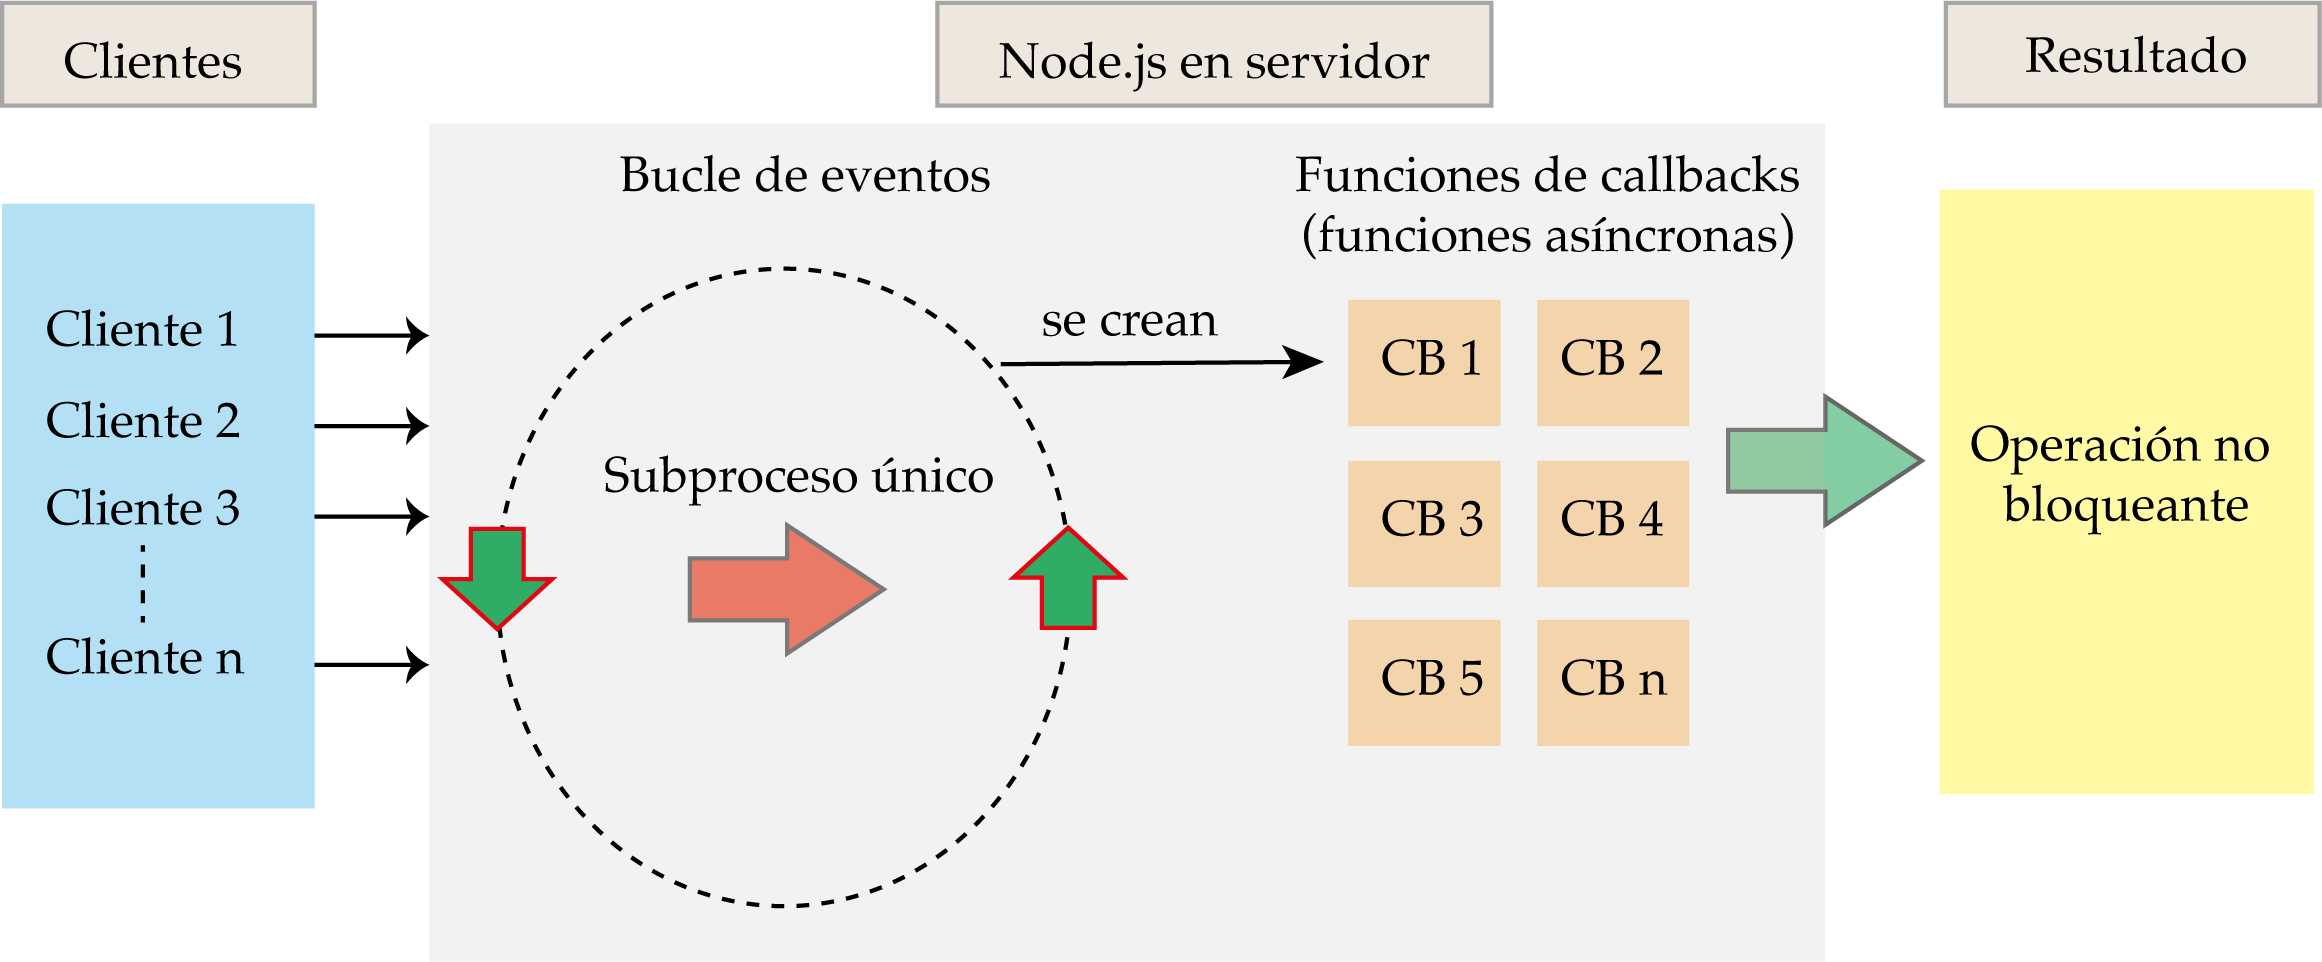
\includegraphics[scale=.65]{./Figures/node-esquema.png}
	\caption[Ejecución de Node.js en servidor ]{Ilustración del proceso de ejecución que realiza Node.js en un servidor.}
	\label{fig:node-esquema}
\end{figure}

Cuando un sistema síncrono ejecuta una llamada, las instrucciones posteriores a esa llamada no se ejecutan hasta que esta ha sido completada. Node.js es un sistema asíncrono. Esto significa que las llamadas y métodos son
ejecutados de forma secuencial, pero sin esperar a que la anterior llamada haya finalizado como se muestra en la figura \ref{fig:sinc-async}. Como conclusión podemos observar que se reduce considerablemente el tiempo de ejecución.

\begin{figure}[htpb]
	\centering
	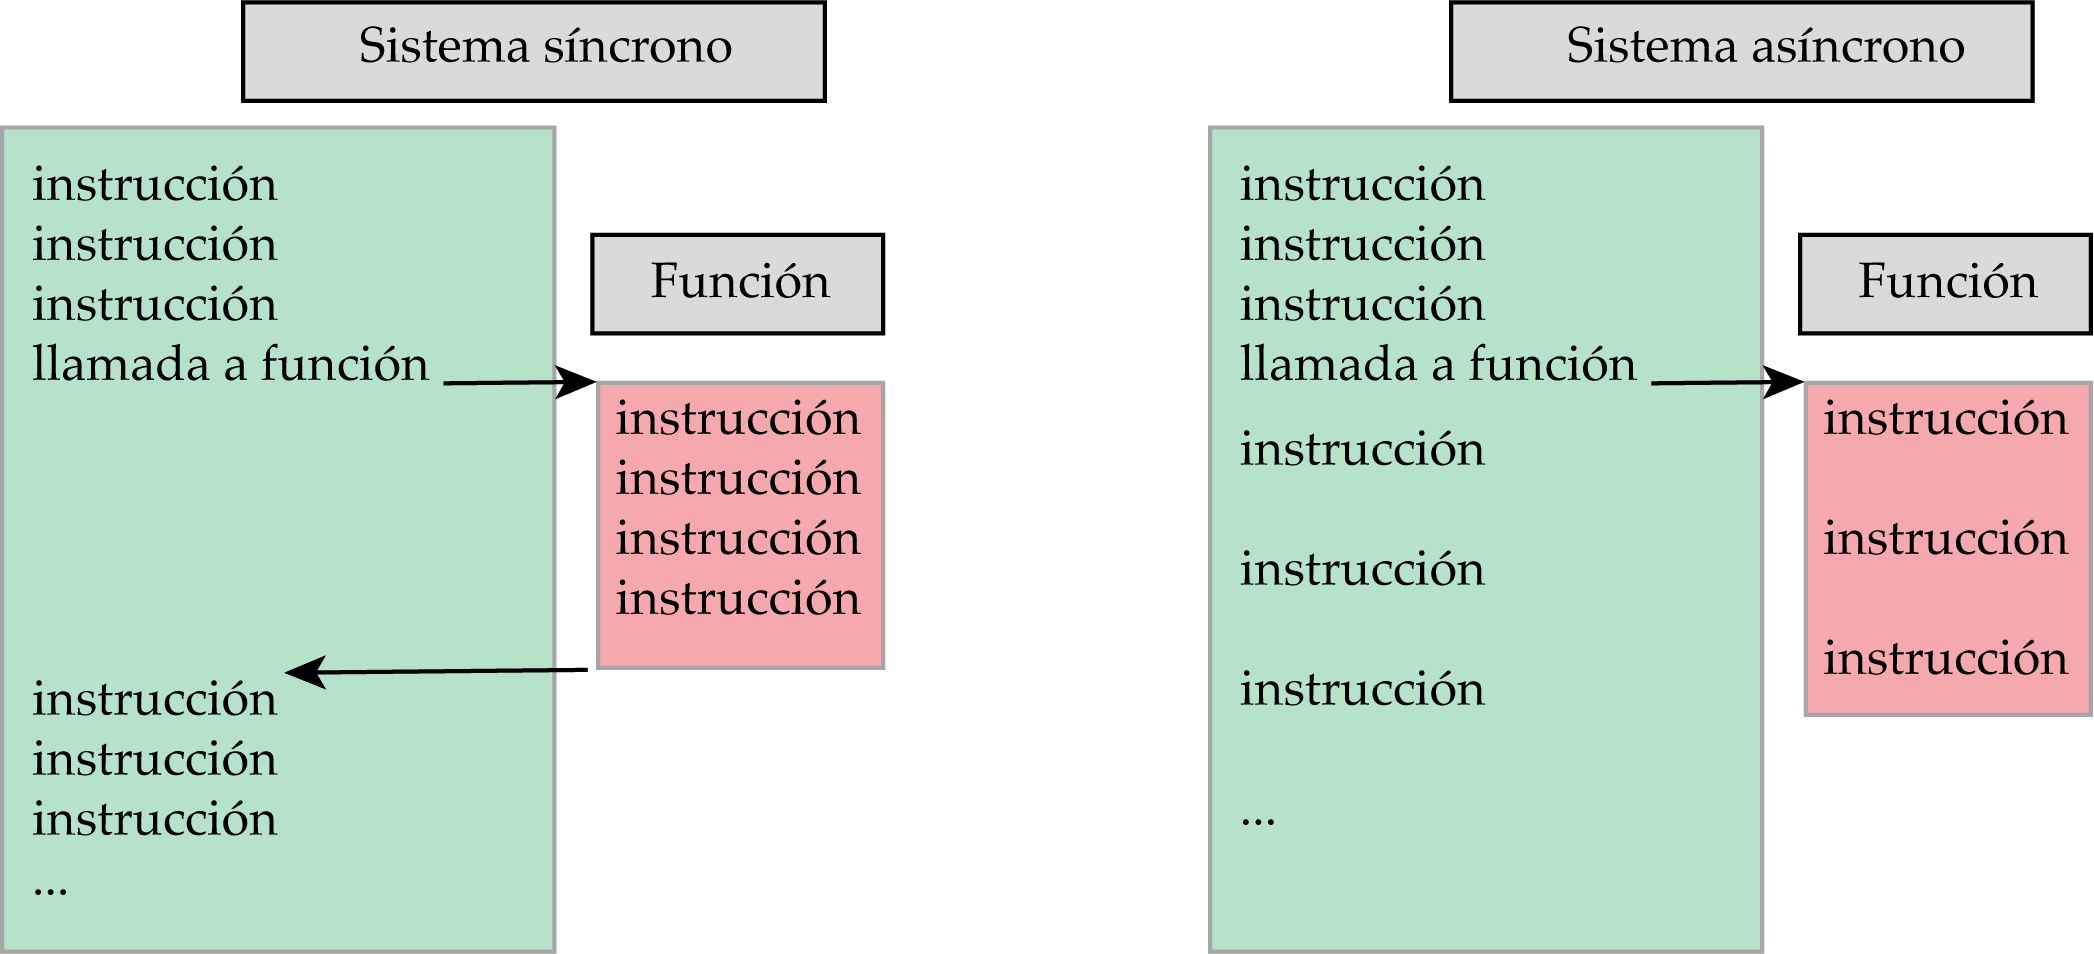
\includegraphics[scale=.65]{./Figures/funciones-asinc.png}
	\caption[Funciones síncronas y asíncronas ]{Ilustración de un sistema síncrono y un sistema asíncrono.}
	\label{fig:sinc-async}
\end{figure}


%----------------------------------------------------------------------------------------
%	SECTION {Mongo}
%----------------------------------------------------------------------------------------
\subsection{Base de datos MongoDB}

MongoDB es una base de datos noSQL\citep{WEBSITE:22},  donde se puede agregar información en forma de documentos en vez de registros como es el caso de las bases de datos SQL\citep{WEBSITE:23}.  La principal ventaja de esta base de datos noSQL es la velocidad de consulta, el motivo de esto es porque la información se la almacena en archivos de formato BSON que son versiones modificadas de JSON. 

Las características principales de MongoDB son:

\begin{itemize}
	\item Escalabilidad horizontal: MongoDB está diseñado para escalar de manera ilimitada a lo que otras bases de datos no podrían, a través de su replicación \citep{WEBSITE:24} y su \textit{sharding}\citep{WEBSITE:25} se puede almacenar información de varios equipos conectados entre sí.
	
	\item Consultas Ad hoc: permite la consulta de información a través de búsquedas de campos,
expresiones regulares con comandos de manera rápida y eficaz.

	\item Indexación: MongoDB utiliza indexación para aumentar la eficiencia en la búsqueda de
información.

	\item Replicación: MongoDB puede realizar replicación maestro – esclavo. El maestro ejecuta comandos para la lectura y escritura de los datos mientras que el esclavo realiza solo lectura de datos pero no los puede modificar.
	
	\item Distribución de carga: MongoDB permite que pueda ejecutarse en distintos servidores a la vez, haciendo más fácil su distribución en la carga de usuarios que deseen conectarse así como acceder a la información. 
	
\end{itemize}




Algunos comandos para el manejo de MongoDB se pueden observar en la tabla \ref{tab:mongo-commands}.  Normalmente en las bases de datos, se mencionan operaciones CRUD,  del acrónimo de "Crear, Leer, Actualizar y Borrar"(del original en ingles \textit{Create}, \textit{Read}, \textit{Insert} y \textit{Delete}) y se usa para referirse a las funciones básicas para el manejo de la información. Para el caso de MongoDB,  estas palabras se reemplazan por \textit{Insert}, \textit{Find}, \textit{Update} y \textit{Remove} respectivamente.

\begin{table}[h]
	\centering
	\caption[Comandos utilizados en MongoDB]{Comandos mas utilizados para el manejo de base de datos que utiliza MongoDB.}
	\begin{tabular}{l l }    
		\toprule
		\textbf{Comando} 	 & \textbf{Descripción} 		\\
		\midrule
	
		\textit{use} 							& Crear una nueva base de dato o utilizar una existente.\\		
		\textit{insertOne}					& Crear un documento en una colección determinada.\\	
		\textit{count}						& Cuenta la cantidad de documentos que hay en una colección.\\	
		\textit{drop}							& Elimina una colección de la base de datos.\\	
		\textit{find	} 						& Se busca un documento en una colección\\
		\textit{remove}	 					& Elimina un documento de una colección\\
		\textit{update}						& Modifica un documento de una colección\\
		
		\bottomrule
		\hline
	\end{tabular}
	\label{tab:mongo-commands}
\end{table}

MongoDB almacena los documentos creados en colecciones que son el análogo a tablas en base de datos relacionales.  En la figura \ref{fig:tabla-coleccion} se ejemplifica la analogía entre tablas en base de datos relacionales y colecciones en MongoDB.

\begin{figure}[htpb]
	\centering
	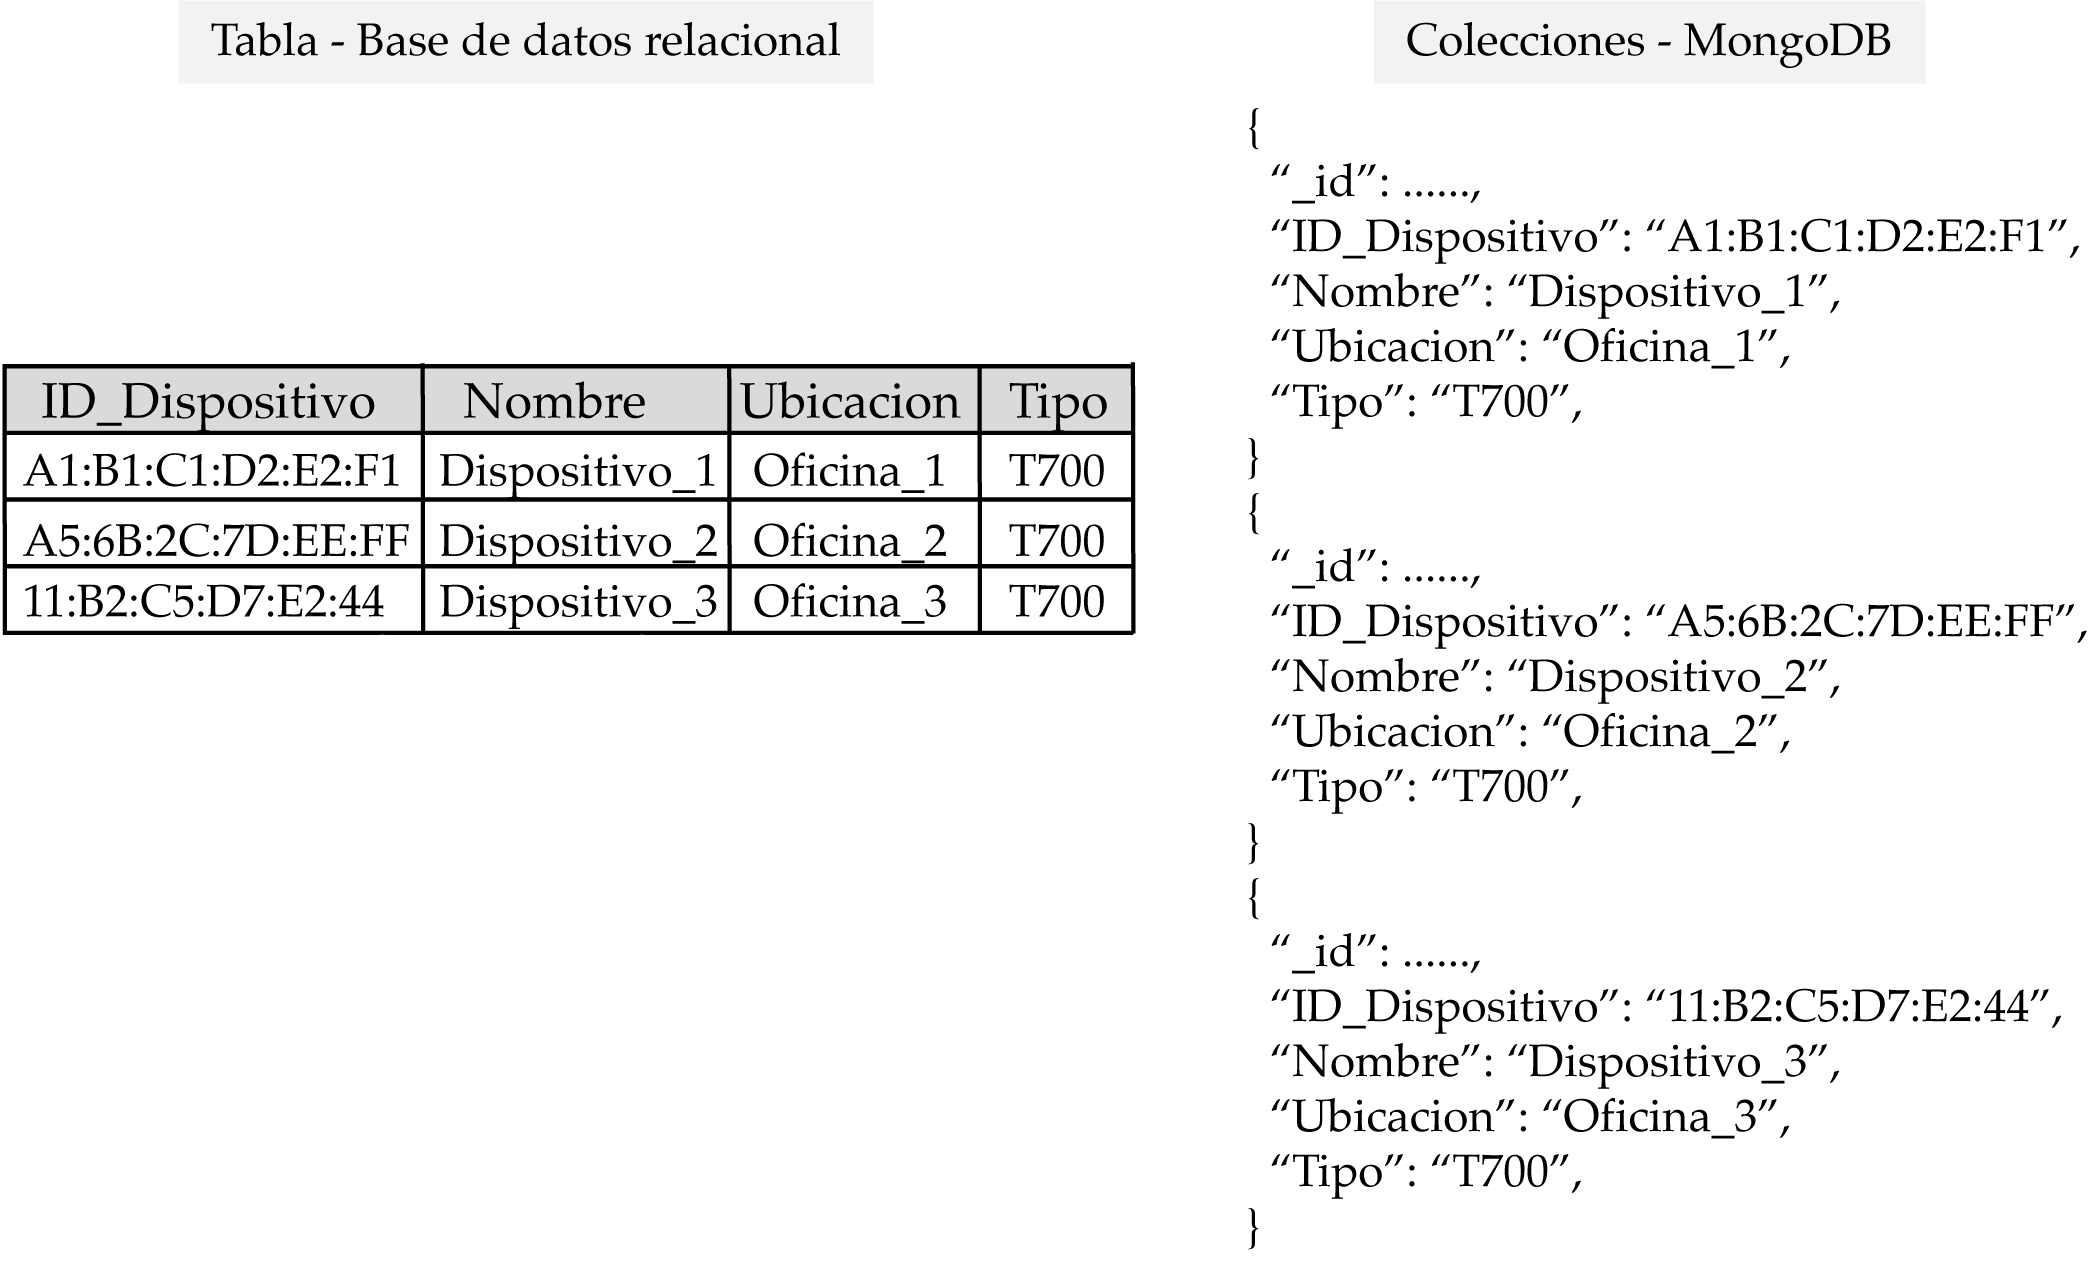
\includegraphics[scale=.7]{./Figures/tabla-coleccion.png}
	\caption[Comparación tabla - colecciones en MongoDB ]{Ilustración de analogía entre tablas en base de datos relacionales y colecciones en MongoDB.}
	\label{fig:tabla-coleccion}
\end{figure}




%----------------------------------------------------------------------------------------
%	SECTION {FrontEnd}
%----------------------------------------------------------------------------------------
\section{Infraestructura del frontend}

Frontend es la parte de un programa o dispositivo a la que un usuario puede acceder directamente. Son todas las tecnologías de diseño y desarrollo web que se ejecutan en el navegador y que se encargan de la interacción con los usuarios.  Se desarrolla, principalmente, a través de tres lenguajes: HTML (\textit{HyperText Markup Language}), CSS (\textit{Cascading Style Sheets})\citep{WEBSITE:26} y JS (Javascript)\citep{WEBSITE:27} . Cada uno de estos lenguajes se usa para desarrollar diferentes partes del frontend.  Estos lenguajes de programación se dividen en tres tareas básicas del desarrollo:

\begin{itemize}
	\item Arquitectura: HTML es el componente mas importante de cualquier proceso de desarrollo de sitios web y proporciona un marco general de cómo se verá el mismo. Es un lenguaje de marcado que nos permite indicar la estructura de nuestro documento mediante etiquetas. Este lenguaje ofrece una gran adaptabilidad, una estructuración lógica y es fácil de interpretar tanto por humanos como por máquinas.
	
	\item Apariencia : CSS (en español Hoja de Estilos en Cascada) controla el aspecto de presentación del sitio, una vez que este ya está construido con HTML.  Es un lenguaje de diseño gráfico para definir y crear la presentación de un documento estructurado escrito en un lenguaje de marcado. Está diseñado principalmente para marcar la separación del contenido del documento y la forma de presentación de este.
	
	\item Interacción: JS.  Es un lenguaje de programación basado en eventos que se utiliza para transformar una página estática en una interfaz dinámica interactuando con el usuario, el navegador y el servidor.  JavaScript es un lenguaje de programación interpretado, dialecto del estándar ECMAScript\citep{WEBSITE:28}.  Se define como orientado a objetos, basado en prototipos, imperativo, débilmente tipado y dinámico.
	
\end{itemize}

Para el desarrollo del frontend de este trabajo se utilizó Angular\citep{WEBSITE:29} que es un \textit{framework} de diseño eficiente y sofisticado de plataformas web. 

%----------------------------------------------------------------------------------------
%	SECTION {Angular}
%----------------------------------------------------------------------------------------
\subsection{Angular}

Angular es una plataforma de desarrollo, construida sobre \textit{Typescript}\citep{WEBSITE:30}. Como plataforma, Angular incluye:

\begin{itemize}
	\item Un marco basado en componentes para crear aplicaciones web escalables.
	
	\item Una colección de bibliotecas bien integradas que cubren una amplia variedad de características, que incluyen enrutamiento, administración de formularios, comunicación cliente-servidor, entre otras.
	
	\item Un conjunto de herramientas para desarrolladores que ayudan a desarrollar, compilar, probar y actualizar el código.
	
\end{itemize}

Para crear aplicaciones con Angular, se generan \textit{templates} con HTML y se controlan estos mismos con lógica creada en los componentes, que serán exportados como clases. Así mismo, se agrega lógica en servicios para manejar datos que la aplicación tendrá y finalmente se encapsulan los componentes y servicios en módulos o \textit{NgModules}.

Cuando se inicia la aplicación, lo hace desde el \textit{root module}. Angular toma el control y muestra el contenido en el explorador web, reaccionando a la interacción de los usuarios que utilicen la aplicación de acuerdo a las instrucciones que contiene la lógica programada.

Un módulo o \textit{NgModule} declara un contexto de compilación para un conjunto de componentes. Puede asociar sus componentes con servicios, para formar unidades funcionales. 

Cada aplicación generada con Angular cuenta con un \textit{root module} o módulo de raíz llamado convencionalmente \textit{AppModule}, el cual provee el mecanismo de arranque que inicia la aplicación. Una aplicación contiene varios módulos funcionales, además un módulo puede importar funcionalidades de otros módulos, y exportar sus propias funcionalidades. 

Cada aplicación de Angular tiene al menos un componente. Al igual que el \textit{root module}, existe el \textit{root component} que conecta una jerarquía de componentes con el DOM (\textit{Document Object Model})\citep{WEBSITE:31}.  Cada componente define una clase que contiene datos y lógica, y está vinculada con el archivo HTML.

El binding a propiedades, o \textit{property binding} en inglés, sirve para asignar un valor a una propiedad de un elemento de un \textit{template}. Esa asignación podrá ser un valor literal, escrito tal cual en el \textit{template}, pero generalmente se tratará de un valor obtenido a través de una propiedad del componente, de modo que si el estado del componente cambia, también cambia la propiedad del elemento asignada en el template.

Por otro lado, cuando un usuario interactúa con un enlace, pulsa un botón, selecciona un evento de una lista desplegable o manipula el texto, el binding de eventos o \textit{event binding} permite a una aplicación de Angular ejecutar código y acciones cuando se produce un evento.

Todos los datos o lógica que no está asociada directamente a una vista y que requiera ser utilizada en diferentes partes de la aplicación y entre diferentes componentes, puede ser escrita en un servicio. Al igual que un componente, los servicios son exportados como clases. Los servicios cuentan con el decorador @Injectable() que provee metadata que permite que los servicios sean inyectados en componentes como dependencias.  \textit{Dependency injection} o Inyección de Dependencias permite manejar las clases de los componentes de forma ligera y eficiente. 

El esquema de la figura \ref{fig:esquema-angular} ejemplifica en forma de bloques, el funcionamiento general de Angular.

\begin{figure}[htpb]
	\centering
	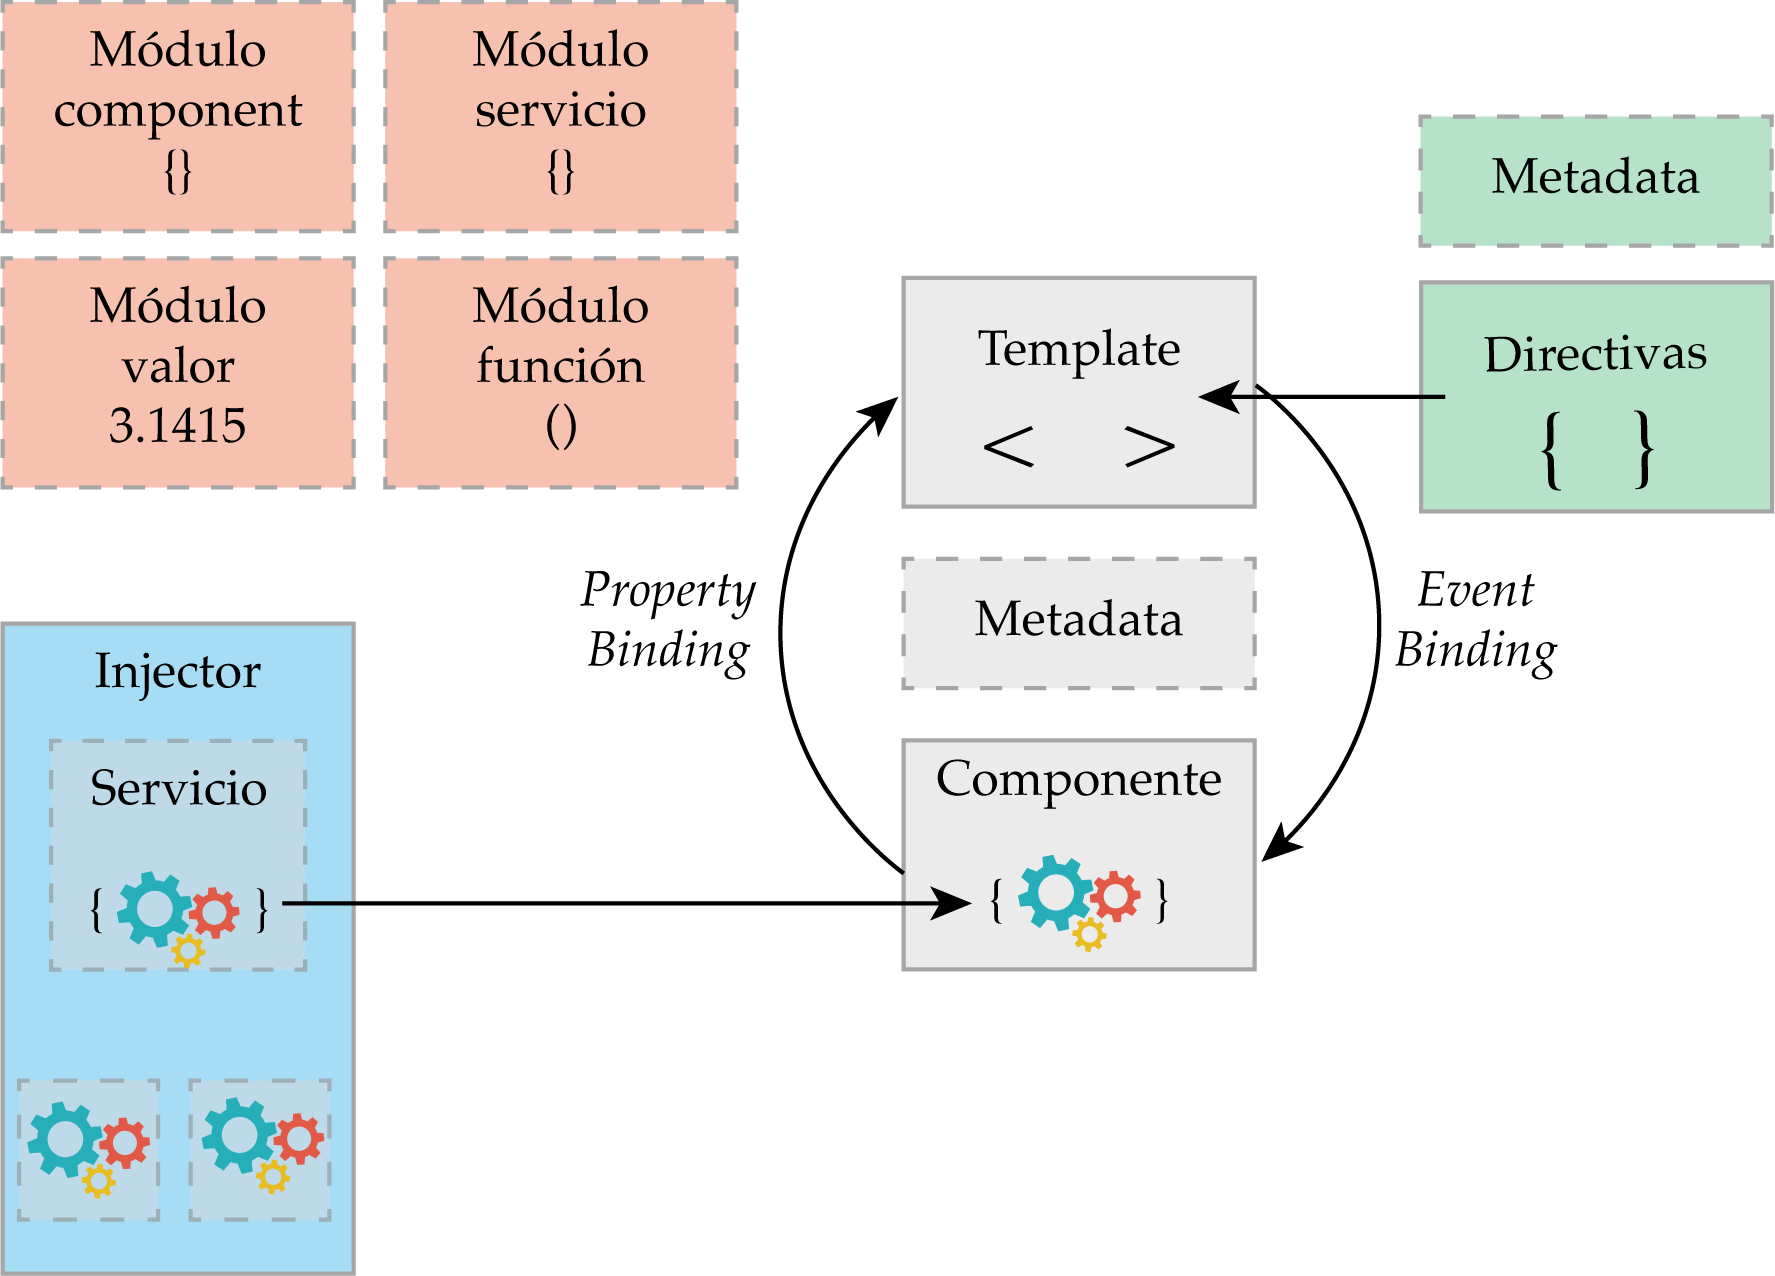
\includegraphics[scale=.7]{./Figures/angular-esquema.png}
	\caption[Arquitectura de funcionamiento de Angular ]{Ilustración de arquitectura de funcionamiento de Angular\protect\footnotemark.}
	\label{fig:esquema-angular}
\end{figure}

\footnotetext{Imagen acondicionada de \url{https://angular.io/guide/architecture}}
%----------------------------------------------------------------------------------------
%	SECTION {Nginx}
%----------------------------------------------------------------------------------------
\section{Servidor Nginx}


Nginx \citep{WEBSITE:32} es un servidor web de código abierto que también es usado como proxy inverso, cache de HTTP, y balanceador de carga.  Es un software modular, lo que significa que las diferentes características son presentadas en forma de módulos y, como administrador, pueden ser activadas o desactivadas. Como consecuencia, el usuario goza de las siguientes características:

\begin{itemize}
	\item \textit{Application Acceleration} (acelerador de aplicaciones), agiliza la entrega de contenidos.
	
	\item Servidor proxy inverso para la aceleración web (HTTP, TCP, UDP) o como proxy de correo electrónico (IMAP, POP3, SMTP).
	
	\item Cifrado TLS para una transferencia de datos segura.
	
	\item Gestión de ancho de banda para un mejor rendimiento.
	
	\item Balanceo de carga con reorientación de solicitudes para disminuir la carga del servidor.
	
\end{itemize}


Nginx trabaja enfocado a eventos. Como consecuencia, puede procesar solicitudes de forma asíncrona, ahorrando memoria y espacio. Este software de servidor es soportado por una gran variedad de sistemas operativos, incluyendo variantes de UNIX / Linux, Mac OS o Windows, fue concebido inicialmente como una respuesta al problema C10K \citep{WEBSITE:33}, que se refiere al problema de rendimiento de manejar 10,000 conexiones concurrentes.

Logra excelentes resultados en el procesamiento de un gran número de solicitudes de los clientes y aprovecha eficazmente los recursos.

Nginx es un servidor asíncrono construido buscando solucionar los problemas de concurrencia que experimentaban ciertos sitios. El algoritmo desarrollado para este servidor es mucho más eficiente y consume menos recursos.

Nginx genera procesos \textit{worker}, cada uno de los cuales puede manejar muchas conexiones. Se puede lograr esto debido a la implementación de un mecanismo de bucle rápido que busca y procesa eventos continuamente. Cada conexión manejada por el \textit{worker} es dispuesta dentro del bucle de eventos, donde vive con otras conexiones. Los eventos dentro de este bucle se procesan de forma asíncrona, permitiendo que el trabajo sea manejado de forma no bloqueante. Cuando una conexión se cierra, se elimina del bucle. Esta disposición asíncrona y monohilos ayuda a que,incluso con recursos limitados, Nginx sea bastante rápido en cuanto al procesamiento de conexiones. Por consiguiente, el uso de CPU y memoria tiende a bajar debido a la eficiencia en el manejo de conexiones. En la figura  \ref{fig:worker-nginx} se ejemplifica el proceso principal de Nginx con la creación de n \textit{workers} por cada consulta / respuesta.

\begin{figure}[htpb]
	\centering
	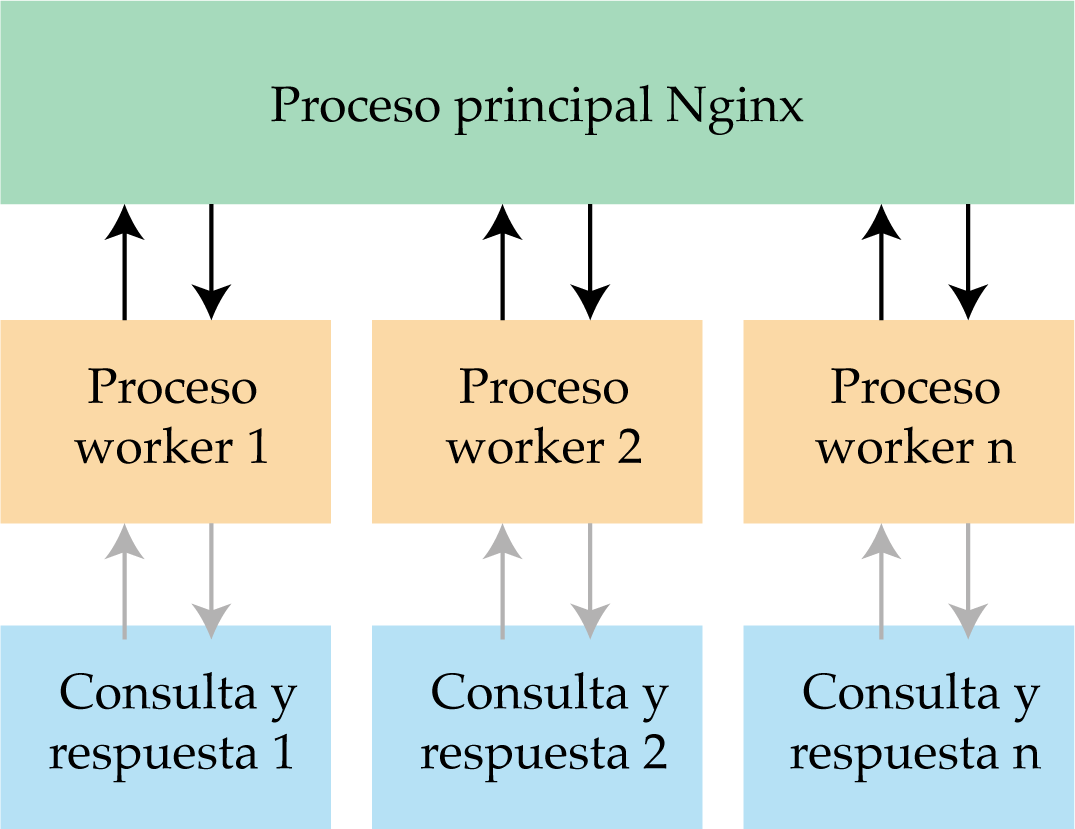
\includegraphics[scale=.7]{./Figures/worker-nginx.png}
	\caption[Proceso principal Nginx ]{Ilustración de funcionamiento principal de Nginx con n consultas / respuestas.}
	\label{fig:worker-nginx}
\end{figure}

Para este trabajo se utilizó Nginx como proxy inverso. Se conoce como proxy inverso cuando un servidor acepta todo el tráfico y lo reenvía a un recurso específico, por ejemplo a una consulta al backend o bien acceder al frontend. El motivo para utilizar un servidor proxy inverso es el agregado de seguridad al servidor principal,  restringir el acceso a rutas definidas y evitar ataques. En la figura \ref{fig:proxy-nginx}  se observa la configuración típica de nginx como proxy inverso, donde se destaca que cada uno de los clientes tendrán un solo punto de acceso a los recursos del servidor. 

\begin{figure}[htpb]
	\centering
	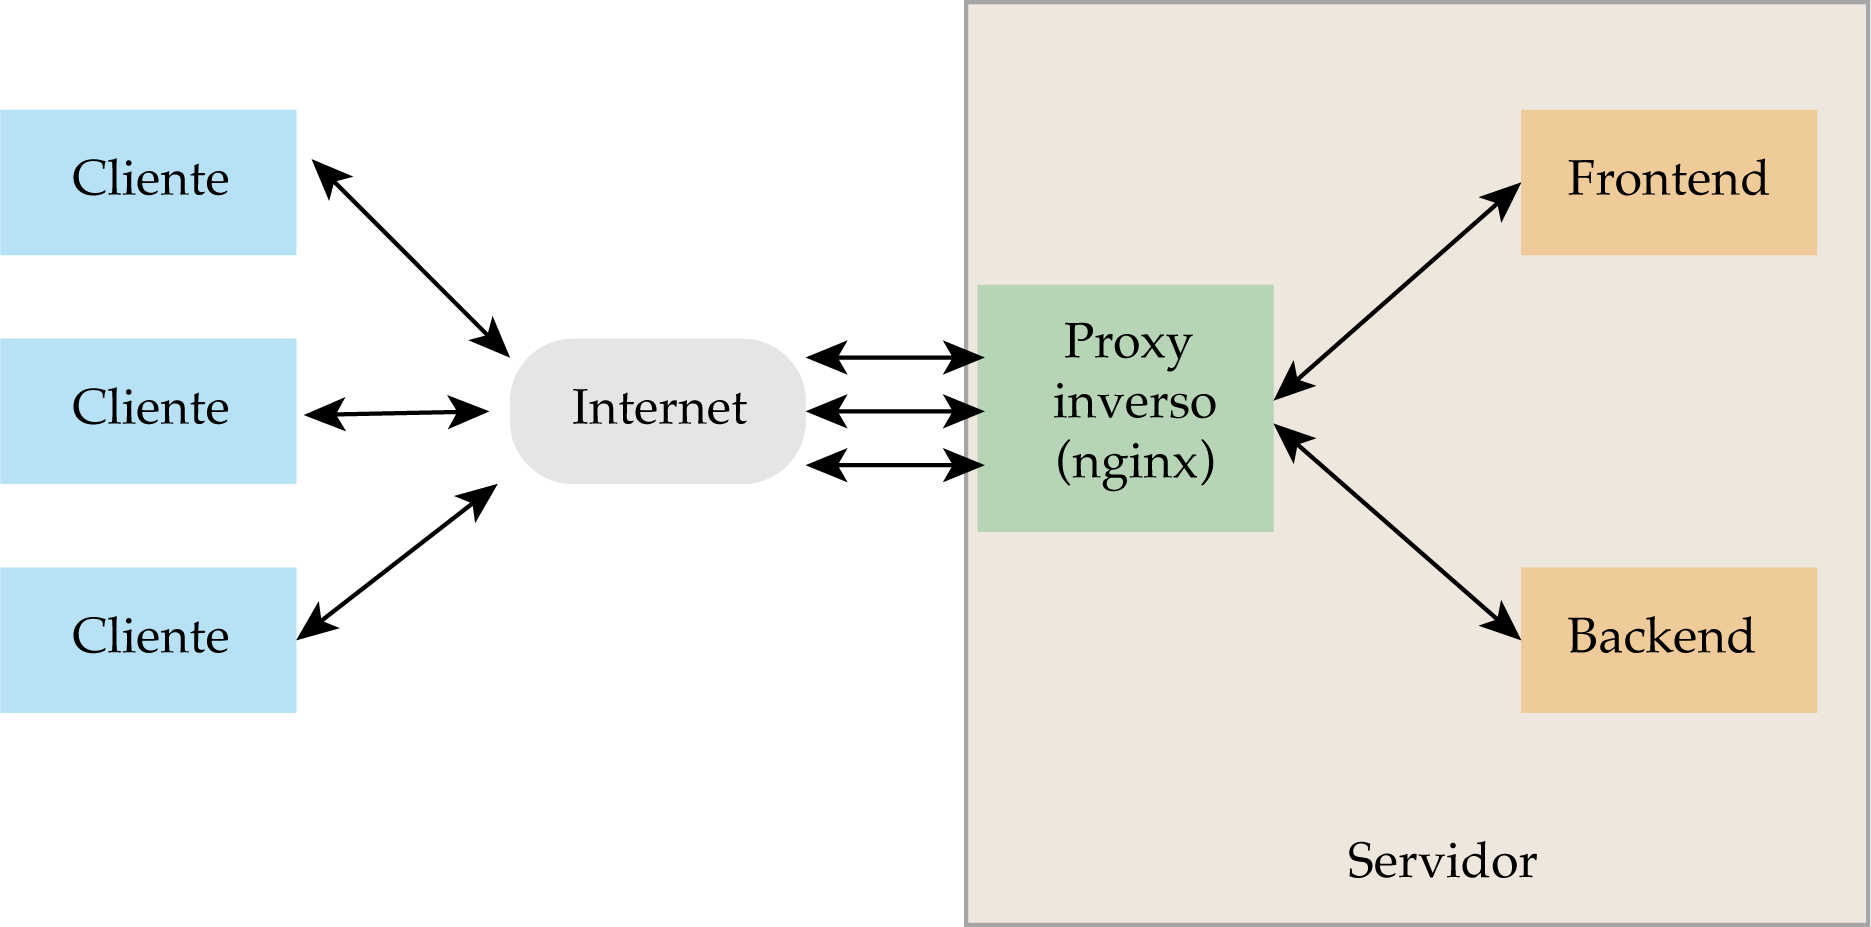
\includegraphics[scale=.7]{./Figures/ngix-proxy.png}
	\caption[Configuración Nginx como proxy inverso ]{Ilustración de configuración de ngix como proxy inverso.}
	\label{fig:proxy-nginx}
\end{figure}



















